\lecturechapter[9]{Dienstag}{21. Apr}{21. April 2026}{Kardinalzahlen und der Satz von Cantor-Bernstein-Schröder}

\begin{nice-box}[Vorlesungsübersicht: Kardinalzahlen und der Satz von Cantor-Bernstein-Schröder]
In der heutigen Vorlesung beschäftigen wir uns mit den Grundlagen der Kardinalzahlarithmetik und den Grenzen der Unendlichkeit. Die Schwerpunkte sind:
\begin{enumerate}[label=\textbf{(\arabic*)}]
    \item \textbf{Das Auswahlaxiom:} Abgeschwächte Formen und historische Einordnung.
    \item \textbf{Gleichmächtigkeit von Mengen:} Definitionen und grundlegende Beispiele.
    \item \textbf{Der Satz von Cantor-Bernstein-Schröder:} Formulierung, Beweis und Anwendungen (z.B. Abzählbarkeit von $\mathbb{Q}$).
    \item \textbf{Der Satz von Cantor:} Warum die Potenzmenge stets mächtiger ist ($|M| < |\mathcal{P}(M)|$).
    \item \textbf{Kardinalzahlen in ZFC:} Definition, Aleph-Notation und die Kontinuumshypothese (CH).
    \item \textbf{Kardinalzahlarithmetik:} Addition, Multiplikation, Potenzierung und die Idempotenzgesetze für unendliche Kardinalzahlen.
\end{enumerate}
\end{nice-box}

\section{Das Auswahlaxiom und seine Bedeutung}

\begin{spoken-clean}[00:00:00 - 00:01:55]
Hallo zusammen, wir fangen an.

Wir hatten letzte Woche --- oder die letzten zwei Wochen --- in der Vorlesung über das Auswahlaxiom gesprochen. Das ist ein wichtiges Thema in der Mathematik, und wir haben gesehen, dass es sich ein bisschen von den anderen Zermelo-Fraenkel-Axiomen unterscheidet. Es ist ein bisschen mehr oder weniger --- weniger intuitiv. Es gibt eben das Wohlordnungsprinzip, das sehr unintuitiv ist, aber dann wiederum das Auswahlaxiom, das eigentlich doch intuitiv ist. Deswegen verwendet man das Auswahlaxiom gerne mit etwas Vorsicht.

Aber wie gesagt: Es ist unabhängig von Zermelo-Fraenkel, und wenn man das Auswahlaxiom annimmt --- also Zermelo-Fraenkel mit dem Auswahlaxiom ---, dann ist das konsistent genau dann, wenn Zermelo-Fraenkel konsistent ist. Das heißt, man macht nichts Gefährlicheres.
\end{spoken-clean}

\begin{spoken-clean}[00:01:55 - 00:05:57]
In der heutigen Mathematik arbeiten fast alle mit dem Auswahlaxiom und nehmen an, dass es gilt. Ansonsten kommt man in sehr exotische Sphären der Mathematik, aber es ist durchaus legitim zu sagen, dass man das Auswahlaxiom nicht annimmt. In der Algebra ist es allerdings fast nicht vorstellbar, das Auswahlaxiom nicht zu haben.

Dann hätte man nicht mehr das Resultat, dass jeder Körper einen algebraischen Abschluss besitzt. Man hätte auch nicht mehr, dass jedes Ideal in einem Ring in einem maximalen Ideal enthalten ist. Und das sind --- nur als zwei Beispiele unter vielen anderen --- Resultate, die man in der algebraischen Geometrie oder der Zahlentheorie, wie man sie heutzutage betreibt, eigentlich fast täglich verwendet.
\end{spoken-clean}

\begin{nice-box}[Abgeschwächte Formen des Auswahlaxioms]
Vielfach wird in Beweisen nicht das volle Auswahlaxiom gebraucht, sondern nur eine abgeschwächte Form davon. Ein paar solcher abgeschwächten Formen des Auswahlaxioms seien hier aufgelistet:
\begin{itemize}
    \item \textbf{C}($\boldsymbol{\omega}$, $\boldsymbol{\infty}$): Jede abzählbare Familie nicht-leerer Mengen hat eine Auswahlfunktion.
    \item \textbf{C}($\boldsymbol{\omega}$, $\boldsymbol{\omega}$): Jede abzählbare Familie nicht-leerer abzählbarer Mengen hat eine Auswahlfunktion.
    \item \textbf{C}($\boldsymbol{\omega}$, $\boldsymbol{<\omega}$): Jede abzählbare Familie nicht-leerer endlicher Mengen hat eine Auswahlfunktion.
    \item \textbf{C}($\boldsymbol{\omega}$, \textbf{a}): Jede abzählbare Familie von zweielementigen Mengen hat eine Auswahlfunktion.
\end{itemize}
\end{nice-box}

\begin{spoken-clean}[00:05:57 - 00:10:07]
Ich wollte aber trotzdem noch erwähnen --- das steht auch kurz im Skript ---: Man kann natürlich fragen, wenn das Auswahlaxiom potenziell unintuitiv oder problematisch erscheint, weshalb verwendet man nicht einfach eine schwächere Version davon? Vielleicht eine schwächere Version, die gerade noch für das reicht, was man machen möchte. Und da gibt es tatsächlich verschiedene abgeschwächte Versionen.

Anstatt beispielsweise anzunehmen, dass jede Familie von nichtleeren Mengen eine Auswahlfunktion besitzt, sagt man einfach: Wir nehmen das nur für abzählbare Familien von nichtleeren Mengen an. Man sagt also: \qt{Alle Familien} ist ein bisschen sehr stark, beschränken wir uns auf abzählbare Familien.

Eine andere Version wäre, zu sagen: Nur Familien von nicht allzu großen Mengen haben eine Auswahlfunktion. Man kann also fordern: Nur abzählbare Familien von höchstens abzählbaren Mengen haben eine Auswahlfunktion. Oder sogar: Nur abzählbare Familien von nichtleeren endlichen Mengen haben eine Auswahlfunktion. Oder noch schwächer: Nur abzählbare Familien von zweielementigen Mengen haben eine Auswahlfunktion. Und so weiter --- da gibt es viele verschiedene Varianten.

Daraus kann man sich natürlich einen Sport machen und untersuchen: Was impliziert wie viel? Was kann man mit einer bestimmten Variante noch beweisen und was nicht mehr? Sind einige von ihnen äquivalent zueinander und welche nicht? Welche sind echt schwächer, welche echt stärker? Aber das ist, denke ich, eine Nischenindustrie für gewisse Gebiete der Logik. Im mathematischen Alltag, wenn man nicht gerade in der Logik arbeitet, stellt man sich diese Fragen meistens nicht.
\end{spoken-clean}

\begin{spoken-clean}[00:10:07 - 00:11:50]
Das andere, was man vielleicht immer ein bisschen im Hinterkopf haben sollte, ist: Wann braucht man das Auswahlaxiom wirklich? Beim Zorn'schen Lemma, das man in der Regel verwendet, ist es relativ klar, wie man es einsetzt, und es ist auch ein bisschen technisch. Das heißt, das wird man wohl kaum verwenden, wenn man es nicht wirklich benötigt.

Beim Auswahlaxiom selbst muss man jedoch genau hinschauen; man braucht es nämlich nicht immer. Sie haben wahrscheinlich gesehen: Wenn man nur endlich viele Mengen hat, dann gibt es immer eine Auswahlfunktion. Dazu braucht man das Auswahlaxiom nicht. Ich hatte in den Übungen auch schon Studierende, die argumentierten: \qt{Sei $X$ eine Menge, gemäß Auswahlaxiom können wir jetzt ein Element aus dieser Menge wählen.} Aber eben: Für die Existenz eines einzelnen Elements in einer einzelnen Menge braucht man garantiert kein Auswahlaxiom! Das wissen wir schon aus der Definition: Da die Menge nicht leer ist, gibt es auch ein Element darin. Für solche Dinge braucht man das Auswahlaxiom also nicht.
\end{spoken-clean}

\begin{spoken-clean}[00:11:50 - 00:13:30]
Oder eben dann die Sache, wenn man noch mehr über die Mengen weiß --- dann kann man oft auch ohne das Auswahlaxiom etwas auswählen. Ich glaube, Fabian hat Ihnen wahrscheinlich das Beispiel mit den Schuhen und den Socken erzählt. Das ist ein sehr gutes Beispiel, um es im Kopf zu behalten: Wenn man eine beliebige Menge von Schuhpaaren hat, ist es kein Problem --- man nimmt einfach aus jedem Paar den rechten Schuh heraus, das geht ganz ohne Auswahlaxiom. Bei Socken geht das jedoch nicht mehr; da braucht man das Auswahlaxiom, weil man zwei Socken --- rechts und links --- nicht voneinander unterscheiden kann.

Gut. So viel noch zum Auswahlaxiom. Heute machen wir weiter mit den Kardinalzahlen. Dazu möchte ich Ihnen noch kurz Georg Cantor vorstellen --- ein sehr wichtiger Mathematiker, vor allem in Bezug auf die Mengenlehre. Er hat von 1845 bis 1918 gelebt, ist in St. Petersburg geboren, kam dann aber nach Deutschland. Er hat sogar zwei Jahre hier an der ETH studiert, ging dann aber für das Ende seines Studiums und das Doktorat nach Deutschland --- nach Berlin und Göttingen. Das waren damals die großen Zentren der Mathematik, nicht die ETH.
\end{spoken-clean}

\begin{spoken-clean}[00:13:30 - 00:15:23]
Er hat damals im 19. Jahrhundert diese ganze Sache mit den Ordinalzahlen und den Kardinalzahlen ins Rollen gebracht. Die Grundideen der Ordinal- und Kardinalzahlen gehen also auf Cantor zurück. Er hat die fundamentale Beobachtung gemacht, dass es verschiedene Unendlichkeiten gibt. Das ist eine der schönsten Einsichten im ersten Jahr des Mathematikstudiums: dass Unendlichkeit nicht gleich Unendlichkeit ist, sondern dass es all diese verschiedenen Stufen gibt. Das hat er damals angerissen, und viele der Dinge, die wir hier besprechen, gehen in ihrer Grundidee auf Cantor zurück.

Seine Ideen sind am Anfang natürlich auf großen Widerstand gestoßen, und zwar aus verschiedenen Richtungen. In der Mathematik gab es viele, die seine Arbeit sehr stark kritisierten --- darunter Kronecker, Poincaré, aber auch Hermann Weyl hier an der ETH und L.E.J. Brouwer sowieso, da Brouwer mit dem Intuitionismus seine ganz eigene Philosophie der Mathematik vertrat. Sie alle haben diese Konstruktionen von all diesen Unendlichkeiten anfangs als mathematisch sehr problematisch eingestuft.

Hinzu kam Kritik von philosophischer Seite: Allen voran fand seltsamerweise sogar Wittgenstein die ganze Mengenlehre höchst problematisch. Er schrieb einmal, das mache die Mathematik kaputt.

Und lustigerweise gab es natürlich auch Widerspruch aus theologischen Kreisen --- insbesondere von den Neoscholastikern. Die Argumentation war wohl: Wenn es nicht nur eine absolute Unendlichkeit gibt, sondern viele verschiedene Unendlichkeiten, dann könnte das der Idee, dass es nur einen einzigen Gott gibt, widersprechen. Obwohl gerade Cantor selbst ein sehr überzeugter protestantischer Christ war, diese theologische Kritik vehement ablehnte und sogar die Auffassung vertrat, dass seine mathematischen Ideen ihm von Gott eingegeben worden seien.

Cantor hat unter dieser heftigen Kritik sehr gelitten. Anscheinend hat er deswegen viele Jahre lang kaum publiziert oder konnte nicht richtig arbeiten, weil ihn das psychisch sehr mitgenommen hat. Am Ende seines Lebens hat er dann aber schlussendlich doch wieder mathematische Arbeiten veröffentlicht.

Er war übrigens auch sonst sehr vielseitig interessiert, unter anderem stark an englischer Literatur. Er war ein leidenschaftlicher Verfechter der Theorie, dass Francis Bacon die Werke von Shakespeare geschrieben habe --- eine These, die von heutigen Literaturwissenschaftlern allerdings weitgehend abgelehnt wird.

So viel zu Georg Cantor --- ein faszinierender Mensch und unendlich wichtig für die moderne Mathematik.
\end{spoken-clean}

\begin{didactic-insight}[Georg Cantor und das Unendliche]
Georg Cantors Entdeckung, dass Unendlichkeit nicht gleich Unendlichkeit ist (z.B. die Überabzählbarkeit der reellen Zahlen im Vergleich zur Abzählbarkeit der natürlichen Zahlen), revolutionierte die Grundlagen der Mathematik. Trotz heftigster, teils persönlicher Anfeindungen durch etablierte zeitgenössische Mathematiker wie Leopold Kronecker setzte sich seine Mengenlehre durch. David Hilbert würdigte Cantors Leistung später mit den berühmten Worten: \qt{Aus dem Paradies, das Cantor uns geschaffen, soll uns niemand vertreiben können.}
\end{didactic-insight}

\section{Einführung in die Kardinalzahlen}

\subsection{Gleichmächtigkeit von Mengen}

\begin{spoken-clean}[00:15:23 - 00:17:00]
Kurze Zeit später wurde seine Theorie dann aber sehr schnell anerkannt --- unter anderem von Hilbert ---, und auch viele seiner früheren Kritiker sahen bald ein, dass diese Mathematik von fundamentaler Bedeutung und nicht mehr wegzudenken ist.

Nun aber zu den Kardinalzahlen. Sie haben bereits die Ordinalzahlen kennengelernt. Ordinalzahlen kann man sich wie das Durchzählen vorstellen: Man zählt einfach immer weiter, geht bis ins Unendliche, konstruiert noch größere Zahlen und fügt immer wieder eins hinzu. Man kann zu jeder Ordinalzahl eine Nachfolger-Ordinalzahl bilden --- das ist quasi die Art und Weise, wie man Mengen wohlordnen kann. Bei den Kardinalzahlen geht es hingegen primär darum, wie viele Elemente eine Menge enthält --- also um die Mächtigkeit von Mengen.

Beginnen wir ganz am Anfang mit der folgenden Definition: Zwei Mengen $A$ und $B$ haben dieselbe Mächtigkeit, falls es eine Bijektion $f \colon A \to B$ gibt. Wir schreiben dafür: $|A| = |B|$. Bis jetzt ist das nur eine Notation; wir werden das später noch präzisieren.
\end{spoken-clean}

\begin{spoken-clean}[00:17:00 - 00:18:44]
Schauen wir uns ein Beispiel an. Wir hatten die Ordinalzahl $\omega + \omega$. Wir wollen nun zeigen, dass $\omega + \omega$ dieselbe Kardinalität wie $\omega$ besitzt. Dazu betrachten wir eine Abbildung von $\omega + \omega$ nach $\omega$. Wir schicken eine darin enthaltene Ordinalzahl $\alpha$ auf $\beta + \beta$, falls $\alpha$ von der Form $\omega + \beta$ ist. Alle Elemente hierin sind entweder in $\omega$ enthalten oder sie sind von der Form $\omega$ plus ein Element aus $\omega$. Wenn $\alpha$ also von der Form $\omega + \beta$ ist, dann schicken wir es einfach auf zweimal dieses Element, also $\beta + \beta$. Und wenn es nicht von dieser Form ist, dann bilden wir es auf $\alpha + \alpha + 1$ ab. Das heißt, die einen werden alle auf gerade Zahlen abgebildet, die anderen alle auf ungerade. Das ist tatsächlich eine Bijektion. Diese zwei Mengen sind somit gleichmächtig.

Vielleicht noch ein paar Bemerkungen: Das erste ist, es gilt immer, dass eine Menge dieselbe Mächtigkeit hat wie sich selbst. Die Identitätsabbildung ist immer eine Bijektion. Und dann haben wir: Falls $A$ gleichmächtig zu $B$ ist, dann ist auch $B$ gleichmächtig zu $A$. Eine Bijektion von $A$ nach $B$ hat eine Inverse, und diese Inverse ist eine Bijektion von $B$ nach $A$. Und das Ganze ist auch transitiv --- also falls $A$ dieselbe Kardinalität hat wie $B$ und $B$ dieselbe Kardinalität wie $C$, dann hat auch $A$ dieselbe Kardinalität wie $C$. Einfach weil Verknüpfungen von Bijektionen wieder Bijektionen sind.
\end{spoken-clean}

\begin{math-stroke}[Gleichmächtigkeit von Mengen]
\begin{definition}[Gleichmächtigkeit]\label[definition]{def:gleichmaechtigkeit}
Zwei Mengen $A$ und $B$ heißen \newterm{gleichmächtig}, falls eine Bijektion $f \colon A \to B$ existiert.
Wir schreiben dafür:
\[
|A| = |B|
\]
\end{definition}

\begin{example}[\texorpdfstring{Gleichmächtigkeit von $\omega + \omega$ und $\omega$}{Gleichmächtigkeit von omega + omega und omega}]\label[example]{ex:omega-plus-omega}
Es gilt:
\[
|\omega + \omega| = |\omega|
\]
\end{example}

\begin{short-proof}[Beweis von \cref{ex:omega-plus-omega}]
Wir definieren die Abbildung $f \colon \omega + \omega \to \omega$ durch:
\[
f(\alpha) := \begin{cases}
\beta + \beta & \text{falls } \alpha = \omega + \beta \\
\alpha + \alpha + 1 & \text{sonst}
\end{cases}
\]
Diese Abbildung $f$ ist eine Bijektion, da sie die Elemente der \newterm{zweiten Hälfte} $\omega + \beta$ auf die geraden Zahlen und die Elemente der \newterm{ersten Hälfte} $\alpha < \omega$ auf die ungeraden Zahlen abbildet.
\end{short-proof}

\begin{remark}[Äquivalenzrelation der Gleichmächtigkeit]\label[remark]{rem:gleichmaechtigkeit-aeq}
Die Gleichmächtigkeit verhält sich wie eine Äquivalenzrelation auf der Klasse aller Mengen (für die formalen Axiome der Reflexivität, Symmetrie und Transitivität siehe \cref{def:aequivalenzrelation-part2} in Woche 2). Es gilt für beliebige Mengen $A, B, C$:
\begin{enumerate}[label=\textbf{(\roman*)}]
    \item \textbf{Reflexivität:} $|A| = |A|$ (mittels der Identitätsabbildung $\id_A \colon A \to A$).
    \item \textbf{Symmetrie:} Falls $|A| = |B|$, so ist $|B| = |A| $ (mittels der Umkehrabbildung $f^{-1} \colon B \to A$).
    \item \textbf{Transitivität:} Falls $|A| = |B|$ und $|B| = |C|$, so ist $|A| = |C|$ (mittels der Komposition $g \circ f \colon A \to C$ für $f \colon A \to B$ und $g \colon B \to C$).
\end{enumerate}
\end{remark}
\end{math-stroke}

\subsection{Vergleich von Kardinalitäten}

\begin{spoken-clean}[00:18:44 - 00:23:33]
Und genau, und in der heutigen Mathematik ist auch noch mehr Notation üblich: Falls es eine injektive Abbildung von $B$ nach $A$ gibt, so schreiben wir, dass die Kardinalität von $B$ kleiner gleich der Kardinalität von $A$ ist. Das bedeutet anschaulich, dass $B$ gleichmächtig zu einer Teilmenge von $A$ ist.

Und dann natürlich: Falls $B$ kleiner gleich $A$ ist, aber $B$ nicht gleichmächtig zu $A$ ist, dann schreiben wir, dass $B$ strikt kleiner ist als $A$.
\end{spoken-clean}

\begin{math-stroke}[Vergleich von Kardinalitäten]
\begin{definition}[Größenvergleich von Kardinalitäten]\label[definition]{def:kardinalitaet-vergleich}
Seien $A$ und $B$ Mengen.
\begin{itemize}
    \item \textbf{Kleiner-gleich:} Wir schreiben \newterm{$|B| \le |A|$}, falls eine Injektion $f \colon B \to A$ existiert (d.h. $B$ ist gleichmächtig zu einer Teilmenge von $A$).
    \item \textbf{Strikt kleiner:} Wir schreiben \newterm{$|B| < |A|$}, falls $|B| \le |A|$, aber $|B| \neq |A|$ gilt.
\end{itemize}
\end{definition}
\end{math-stroke}

\begin{spoken-clean}[00:23:33 - 00:24:22]
Das Nächste, was wir uns anschauen wollen, ist der Satz von Cantor-Bernstein-Schröder --- manchmal auch Schröder-Bernstein-Theorem genannt. Dieser besagt: Wenn $A$ und $B$ Mengen sind, sodass $|A| \le |B|$ und $|B| \le |A|$ gilt, dann folgt daraus $|A| = |B|$. Sie haben also dieselbe Mächtigkeit.

Das ist intuitiv sehr naheliegend, aber es ist a priori keineswegs klar, dass das auch wirklich stimmt. Stellen wir uns vor: Wir haben hier Stühle und hier haben wir Leute. Wir wissen, wir können jede Person einem Stuhl zuordnen, sodass jede Person genau einen Stuhl hat --- wobei vielleicht noch Stühle übrig bleiben. Und es gibt auch eine Möglichkeit, die Stühle den Leuten so zuzuordnen, dass für jeden Stuhl eine Person da ist. Für unendliche Mengen ist es aber keineswegs offensichtlich, dass daraus automatisch die Existenz einer Bijektion folgt. Der Satz besagt nun aber, dass das tatsächlich der Fall ist.

Vielleicht noch kurz zu den Namen: Oft wird er einfach Bernstein-Schröder-, Cantor-Schröder- oder eben Cantor-Bernstein-Schröder-Satz genannt. Ich glaube, Schröder war der Erste, der ihn publiziert hat --- allerdings mit einem fehlerhaften Beweis. Cantor hat ihn etwas später ebenfalls veröffentlicht, ebenfalls mit einem falschen Beweis. Bernstein war schließlich der Erste, der einen völlig korrekten Beweis geliefert hat. So viel zur Historie.

Wie beweist man das nun? Ich erkläre den Beweis ein bisschen anders, als er im Skript steht. Es ist im Grunde genau dieselbe Idee und kein anderer Beweis, aber ich finde ihn im Skript stellenweise etwas umständlich formuliert, obwohl es letztlich exakt dasselbe ist, was wir hier tun.

Wir nehmen also an, dass wir eine Injektion $f$ von $A$ nach $B$ und eine Injektion $g$ von $B$ nach $A$ haben.
\end{spoken-clean}

% \begin{math-stroke}
% \begin{theorem}[Cantor-Bernstein-Schröder]\label[theorem]{thm:cantor-bernstein-schroeder}Seien $A$ und $B$ Mengen. Falls $|A| \le |B|$ und $|B| \le |A|$ gilt, dann ist $|A| = |B|$.\end{theorem}
% \end{math-stroke}

% \begin{spoken-clean}[00:24:22 - 00:26:00]
% Wenn natürlich eine von diesen beiden Abbildungen bereits surjektiv ist, dann sind wir sowieso schon fertig. 

% Was wir jetzt tun, ist Folgendes: Wir definieren eine Menge $E_0$ als $A$ ohne das Bild von $B$ unter $g$. Ich schreibe dafür $g(B)$. Mit $g(B)$ meine ich wirklich die Menge aller Elemente der Form $g(b)$, wobei $b$ in $B$ liegt. Im Skript wird das, glaube ich, mit eckigen Klammern geschrieben, aber es ist klar, was gemeint ist. Wir nehmen also alle Elemente in $A$, die nicht im Bild von $B$ liegen.

% Ich kann das grafisch so veranschaulichen: Wir haben hier die Menge $A$ und hier die Menge $B$. Und wir haben eine Injektion $g$ von $B$ nach $A$, das heißt, wir haben das Bild $g(B)$ in $A$. Unser $E_0$ ist nun alles in $A$ außerhalb dieses Bildes $g(B)$."
% \end{spoken-clean}

% \begin{spoken-clean}[00:26:00 - 00:27:30]
% Nun betrachten wir das Bild von $A$ unter $f$ in $B$, das ist $f(A)$. Und darin liegt das Bild von $E_0$, also $f(E_0)$. Wenn wir nun mit $g$ wieder zurückgehen, erhalten wir die Menge $g(f(E_0))$ in $A$. Diese liegt ganz innerhalb von $g(B)$. Und so können wir immer weitergehen: Wir gehen mit $f$ hinein, mit $g$ zurück, wieder mit $f$ hinein und wieder mit $g$ zurück.

% Wir definieren diese Mengen nun sukzessive weiter: Wir setzen $E_1$ als $g(f(E_0))$ und allgemein $E_{n+1}$ als $g(f(E_n))$. So erhalten wir eine absteigende Folge von immer kleineren Mengen.

% Schließlich definieren wir die Menge $E$ als die Vereinigung all dieser $E_n$.
% \end{spoken-clean}

% \begin{spoken-clean}[00:27:30 - 00:29:10]
% Nun betrachten wir die Elemente, die in $E$ liegen, und diejenigen, die nicht in $E$ liegen. Diese beiden Gruppen müssen wir unterschiedlich handhaben. Wir definieren nun direkt eine Abbildung $h$ von $A$ nach $B$ und zeigen, dass sie eine Bijektion ist. Wir definieren $h(x)$ wie folgt: Es soll gleich $f(x)$ sein, falls $x$ in dieser Menge $E$ enthalten ist. Und wenn $x$ nicht in $E$ liegt, dann nehmen wir einfach das Urbild unter $g$, also $g^{-1}(x)$.

% Wir müssen prüfen, ob das überhaupt wohldefiniert ist. Wenn $x$ in $E$ liegt, ist das klar. Wenn $x$ nicht in $E$ liegt, ist es insbesondere nicht in $E_0$ enthalten. Und wenn es nicht in $E_0$ liegt, dann bedeutet das nach Definition von $E_0$, dass es im Bild von $g$ liegen muss, da $E_0$ ja gerade das Komplement des Bildes von $B$ ist. Das heißt, $x$ ist im Bild $g(B)$ enthalten, und somit existiert ein Urbild unter $g$. Da $g$ injektiv ist, ist dieses Urbild auch eindeutig bestimmt. Das heißt, $h$ ist tatsächlich eine wohldefinierte Funktion.
% \end{spoken-clean}

% \begin{spoken-clean}[00:29:10 - 00:30:49]
% Als Nächstes müssen wir zeigen, dass $h$ injektiv ist. Wenn wir die Abbildung auf $E$ einschränken und auf das Komplement von $E$, dann ist das jeweils injektiv, weil $f$ injektiv ist und jedes Element im Komplement von $E$ ein eindeutiges Urbild besitzt --- die Einschränkungen von $h$ auf $E$ und auf $A \setminus E$ sind also injektiv. Wir müssen folglich nur zeigen, dass kein Element aus $E$ auf dasselbe Element abgebildet wird wie ein Element außerhalb von $E$.

% Nehmen wir also an, dass $f(x_1) = g^{-1}(x_2)$ gilt für ein $x_1 \in E$ und ein $x_2 \notin E$. Da $x_1 \in E$ ist, existiert ein $n \in \omega$ mit $x_1 \in E_n$. Daraus folgt aber $g(f(x_1)) = x_2$. Da $x_1 \in E_n$ ist, ist $g(f(x_1))$ nach Definition in $E_{n+1}$ enthalten. Das bedeutet jedoch, dass $x_2 \in E_{n+1} \subseteq E$ gilt --- ein Widerspruch zur Annahme, dass $x_2 \notin E$ ist. Dieser Fall kann also nicht eintreffen, und $h$ ist tatsächlich injektiv.

% Nun müssen wir noch zeigen, dass $h$ surjektiv ist. Dazu nehmen wir ein $y \in B$. Wir wollen zeigen, dass ein Urbild von $y$ unter $h$ existiert. Falls $g(y) \in E$ ist, dann existiert ein $n \in \omega$ mit $g(y) \in E_n$. Da $g(y) \in g(B)$ ist, kann $g(y)$ nicht in $E_0$ liegen, also ist $n \ge 1$. Es gilt also $g(y) \in E_n = g(f(E_{n-1}))$. Da $g$ injektiv ist, folgt daraus sofort $y = f(x)$ für ein $x \in E_{n-1} \subseteq E$. Für dieses $x$ gilt dann $h(x) = f(x) = y$. Falls andererseits $g(y) \notin E$ ist, dann wählen wir einfach $x = g(y) \notin E$. Nach Definition von $h$ gilt dann $h(x) = g^{-1}(x) = g^{-1}(g(y)) = y$. In beiden Fällen finden wir also ein Urbild, und $h$ ist somit surjektiv.

% Das ist in der Praxis natürlich äußerst praktisch, um zu zeigen, dass zwei Mengen gleichmächtig sind. Es ist nämlich oft sehr mühsam, eine explizite Bijektion direkt zu konstruieren. Es ist viel einfacher, stattdessen zwei Injektionen zu finden.
% \end{spoken-clean}

% \begin{math-stroke}[Beweis des Cantor-Bernstein-Schröder-Theorems]
% \begin{short-proof}
% Seien $f \colon A \to B$ und $g \colon B \to A$ injektive Abbildungen.
% Wir definieren rekursiv eine Folge von Teilmengen von $A$:
% \begin{align*}
% E_0 &:= A \setminus g(B) \\
% E_{n+1} &:= g(f(E_n)) \quad \text{für alle } n \in \omega
% \end{align*}
% Sei $E$ die Vereinigung dieser Mengen:
% \[
% E := \bigcup_{n \in \omega} E_n
% \]
% Wir definieren die Abbildung $h \colon A \to B$ durch:
% \[
% h(x) := \begin{cases}
% f(x) & \text{falls } x \in E \\
% g^{-1}(x) & \text{falls } x \notin E
% \end{cases}
% \]

% \begin{center}
% \begin{tikzpicture}[scale=1.2, >=stealth]
%   % \begin{ai-tikz-planner-invisible-content}
%   % 1. Background: Zwei Rechtecke für die Mengen A und B.
%   % 2. Midground: Darstellung des Bildes g(B) in A und die Partitionierung von A in E_0, E_1, E_2...
%   % 3. Foreground: Die Abbildungen f und g als gerichtete Pfeile zwischen den entsprechenden Teilmengen.
%   % \end{ai-tikz-planner-invisible-content}
  
%   % Set A (left box)
%   \draw[thick, MidnightBlue] (0,0) rectangle (3,4) node[above=4cm, midway] {$A$};
%   % Set B (right box)
%   \draw[thick, ForestGreen] (6,0) rectangle (9,4) node[above=4cm, midway] {$B$};

%   % Subsets in A
%   \draw[dashed, MidnightBlue] (0, 3) -- (3, 3);
%   \node at (1.5, 3.5) {$E_0 = A \setminus g(B)$};

%   \draw[dashed, MidnightBlue] (0, 2) -- (3, 2);
%   \node at (1.5, 2.5) {$E_1 = g(f(E_0))$};

%   \draw[dashed, MidnightBlue] (0, 1) -- (3, 1);
%   \node at (1.5, 1.5) {$E_2 = g(f(E_1))$};
%   \node at (1.5, 0.5) {$\vdots$};

%   % Subsets in B
%   \draw[dashed, ForestGreen] (6, 2.5) -- (9, 2.5);
%   \node at (7.5, 3.25) {$f(E_0)$};

%   \draw[dashed, ForestGreen] (6, 1.5) -- (9, 1.5);
%   \node at (7.5, 2.0) {$f(E_1)$};
%   \node at (7.5, 0.75) {$\vdots$};

%   % Mapping arrows
%   \draw[->, thick, BrickRed] (3, 3.5) to[bend left=15] node[midway, above] {$f$} (6, 3.25);
%   \draw[->, thick, BurntOrange] (6, 3.25) to[bend left=15] node[midway, below] {$g$} (3, 2.5);
%   \draw[->, thick, BrickRed] (3, 2.5) to[bend left=15] node[midway, above] {$f$} (6, 2.0);
%   \draw[->, thick, BurntOrange] (6, 2.0) to[bend left=15] node[midway, below] {$g$} (3, 1.5);
% \end{tikzpicture}
% \end{center}

% \textbf{1. Wohldefiniertheit von $h$:}
% Falls $x \notin E$, so ist insbesondere $x \notin E_0 = A \setminus g(B)$. Daraus folgt $x \in g(B)$. Da $g$ injektiv ist, existiert ein eindeutiges Urbild $g^{-1}(x) \in B$. Somit ist $h$ wohldefiniert.

% \textbf{2. Injektivität von $h$:}
% Seien $x_1, x_2 \in A$ mit $h(x_1) = h(x_2)$.
% \begin{itemize}
%     \item \textbf{Fall 1 ($x_1, x_2 \in E$):} Es gilt $f(x_1) = f(x_2) \implies x_1 = x_2$ (da $f$ ist injektiv).
%     \item \textbf{Fall 2 ($x_1, x_2 \notin E$):} Es gilt $g^{-1}(x_1) = g^{-1}(x_2) \implies x_1 = x_2$ (da $g$ ist injektiv).
%     \item \textbf{Fall 3 (Mischfall):} Angenommen, $x_1 \in E$ und $x_2 \notin E$. Dann gilt $f(x_1) = g^{-1}(x_2) \implies g(f(x_1)) = x_2$. Da $x_1 \in E$, existiert ein $n \in \omega$ mit $x_1 \in E_n$. Daraus folgt $x_2 = g(f(x_1)) \in E_{n+1} \subseteq E$, was im Widerspruch zu $x_2 \notin E$ steht.
% \end{itemize}
% Somit ist $h$ injektiv.

% \textbf{3. Surjektivität von $h$:}
% Sei $y \in B$. Wir suchen ein $x \in A$ mit $h(x) = y$.
% \begin{itemize}
%     \item \textbf{Fall 1 ($g(y) \in E$):} Dann existiert ein $n \in \omega$ mit $g(y) \in E_n$. Da $g(y) \in g(B)$, kann $g(y)$ nicht in $E_0$ liegen, also ist $n \ge 1$. Es gilt $g(y) \in E_n = g(f(E_{n-1}))$. Da $g$ injektiv ist, folgt $y = f(x)$ für ein $x \in E_{n-1} \subseteq E$. Für dieses $x$ gilt $h(x) = f(x) = y$.
%     \item \textbf{Fall 2 ($g(y) \notin E$):} Wir wählen $x := g(y) \notin E$. Dann gilt $h(x) = g^{-1}(x) = g^{-1}(g(y)) = y$.
% \end{itemize}
% Somit ist $h$ surjektiv und folglich eine Bijektion. Es gilt $|A| = |B|$.
% \end{short-proof}
% \end{math-stroke}

% \begin{didactic-insight}[Die Eleganz des Cantor-Bernstein-Schröder-Theorems]
% Der Beweis des Cantor-Bernstein-Schröder-Theorems ist ein klassisches Beispiel für ein nicht-konstruktives Auswahlverfahren in der Mengenlehre. Anstatt eine explizite Bijektion mühsam von Hand zu definieren --- was bei unendlichen Mengen oft unmöglich ist ---, erlaubt uns der Satz, das Problem auf das Auffinden zweier Injektionen $f \colon A \to B$ und $g \colon B \to A$ zu reduzieren. Die Funktion $h$ partitioniert die Menge $A$ geschickt in Ketten von Vor- und Nachbildern, um lokale Bijektionen zusammenzuflicken.
% \begin{align*}
%   A &= E \;\dot{\cup}\; (A \setminus E) \\
%   B &= f(E) \;\dot{\cup}\; (B \setminus f(E))
% \end{align*}
% Auf $E$ verwenden wir die ``Vorwärtsabbildung'' $f$, auf dem Komplement $A \setminus E$ die ``Rückwärtsabbildung'' $g^{-1}$.
% \end{didactic-insight}


% \begin{math-stroke}
% \begin{theorem}[Cantor-Bernstein-Schröder]\label[theorem]{thm:cantor-bernstein-schroeder}
% Seien $A$ und $B$ Mengen. Falls $|A| \le |B|$ und $|B| \le |A|$ gilt, dann ist $|A| = |B|$.
% \end{theorem}
% \end{math-stroke}

% \begin{spoken-clean}[00:24:22 - 00:26:00]
% Wenn natürlich eine von diesen beiden Abbildungen bereits surjektiv ist, dann sind wir sowieso schon fertig. 

% Was wir jetzt tun, ist Folgendes: Wir definieren eine Menge $E_0$ als $A$ ohne das Bild von $B$ unter $g$ (also $A \setminus g(B)$). Ich schreibe dafür $g(B)$. Mit $g(B)$ meine ich wirklich die Menge aller Elemente der Form $g(b)$, wobei $b$ in $B$ liegt. Im Skript wird das, glaube ich, mit eckigen Klammern geschrieben (als $g[B]$), aber es ist klar, was gemeint ist. Wir nehmen also alle Elemente in $A$, die nicht im Bild von $B$ liegen.

% Ich kann das grafisch so veranschaulichen: Wir haben hier die Menge $A$ und hier die Menge $B$. Und wir haben eine Injektion $g$ von $B$ nach $A$, das heißt, wir haben das Bild $g(B)$ in $A$. Unser $E_0$ ist nun alles in $A$ außerhalb dieses Bildes $g(B)$.
% \end{spoken-clean}

% \begin{spoken-clean}[00:26:00 - 00:27:30]
% Nun betrachten wir das Bild von $A$ unter $f$ in $B$, das ist $f(A)$. Und darin liegt das Bild von $E_0$, also $f(E_0)$. Wenn wir nun mit $g$ wieder zurückgehen, erhalten wir die Menge $g(f(E_0))$ in $A$. Diese liegt ganz innerhalb von $g(B)$. Und so können wir immer weitergehen: Wir gehen mit $f$ hinein, mit $g$ zurück, wieder mit $f$ hinein und wieder mit $g$ zurück.

% Wir definieren diese Mengen nun sukzessive weiter: Wir setzen $E_1$ als $g(f(E_0))$ und allgemein $E_{n+1}$ als $g(f(E_n))$. So erhalten wir eine absteigende Folge von immer kleineren Mengen (die eine Kette bilden).

% Schließlich definieren wir die Menge $E$ als die Vereinigung all dieser $E_n$.
% \end{spoken-clean}

% \begin{spoken-clean}[00:27:30 - 00:29:10]
% Nun betrachten wir die Elemente, die in $E$ liegen, und diejenigen, die nicht in $E$ liegen (also $A \setminus E$). Diese beiden Gruppen müssen wir unterschiedlich handhaben. Wir definieren nun direkt eine Abbildung $h$ von $A$ nach $B$ und zeigen, dass sie eine Bijektion ist. Wir definieren $h(x)$ wie folgt: Es soll gleich $f(x)$ sein, falls $x$ in dieser Menge $E$ enthalten ist. Und wenn $x$ nicht in $E$ liegt, dann nehmen wir einfach das Urbild unter $g$, also $g^{-1}(x)$.

% Wir müssen prüfen, ob das überhaupt wohldefiniert ist. Wenn $x$ in $E$ liegt, ist das klar. Wenn $x$ nicht in $E$ liegt, ist es insbesondere nicht in $E_0$ enthalten. Und wenn es nicht in $E_0$ liegt, dann bedeutet das nach Definition von $E_0$, dass es im Bild von $g$ liegen muss, da $E_0$ ja gerade das Komplement des Bildes von $B$ ist. Das heißt, $x$ ist im Bild $g(B)$ enthalten, und somit existiert ein Urbild unter $g$. Da $g$ injektiv ist, ist dieses Urbild auch eindeutig bestimmt. Das heißt, $h$ ist tatsächlich eine wohldefinierte Funktion.
% \end{spoken-clean}

% \begin{spoken-clean}[00:29:10 - 00:30:49]
% Als Nächstes müssen wir zeigen, dass $h$ injektiv ist. Wenn wir die Abbildung auf $E$ einschränken und auf das Komplement von $E$, dann ist das jeweils injektiv, weil $f$ injektiv ist und jedes Element im Komplement von $E$ ein eindeutiges Urbild besitzt --- die Einschränkungen von $h$ auf $E$ und auf $A \setminus E$ sind also injektiv. Wir müssen folglich nur zeigen, dass kein Element aus $E$ auf dasselbe Element abgebildet wird wie ein Element außerhalb von $E$.

% Nehmen wir also an, dass $f(x_1) = g^{-1}(x_2)$ gilt für ein $x_1 \in E$ und ein $x_2 \notin E$ (ein sogenannter Mischfall). Da $x_1 \in E$ ist, existiert ein $n \in \omega$ mit $x_1 \in E_n$. Daraus folgt aber $g(f(x_1)) = x_2$. Da $x_1 \in E_n$ ist, ist $g(f(x_1))$ nach Definition in $E_{n+1}$ enthalten. Das bedeutet jedoch, dass $x_2 \in E_{n+1} \subseteq E$ gilt --- ein Widerspruch zur Annahme, dass $x_2 \notin E$ ist. Dieser Fall kann also nicht eintreffen, und $h$ ist tatsächlich injektiv.

% Nun müssen wir noch zeigen, dass $h$ surjektiv ist. Dazu nehmen wir ein $y \in B$. Wir wollen zeigen, dass ein Urbild von $y$ unter $h$ existiert. Falls $g(y) \in E$ ist, dann existiert ein $n \in \omega$ mit $g(y) \in E_n$. Da $g(y) \in g(B)$ ist, kann $g(y)$ nicht in $E_0$ liegen, also ist $n \ge 1$. Es gilt also $g(y) \in E_n = g(f(E_{n-1}))$. Da $g$ injektiv ist, folgt daraus sofort $y = f(x)$ für ein $x \in E_{n-1} \subseteq E$. Für dieses $x$ gilt dann $h(x) = f(x) = y$. Falls andererseits $g(y) \notin E$ ist, dann wählen wir einfach $x = g(y) \notin E$. Nach Definition von $h$ gilt dann $h(x) = g^{-1}(x) = g^{-1}(g(y)) = y$. In beiden Fällen finden wir also ein Urbild, und $h$ ist somit surjektiv.

% Das ist in der Praxis natürlich äußerst praktisch, um zu zeigen, dass zwei Mengen gleichmächtig sind. Es ist nämlich oft sehr mühsam, eine explizite Bijektion direkt zu konstruieren. Es ist viel einfacher, stattdessen zwei Injektionen zu finden.
% \end{spoken-clean}

% \begin{math-stroke}[Beweis des Cantor-Bernstein-Schröder-Theorems]
% \begin{short-proof}
% Seien $f \colon A \to B$ und $g \colon B \to A$ injektive Abbildungen.
% Wir definieren rekursiv eine Folge von Teilmengen von $A$:
% \begin{align*}
% E_0 &:= A \setminus g(B) \\
% E_{n+1} &:= g(f(E_n)) \quad \text{für alle } n \in \omega
% \end{align*}
% Sei $E$ die Vereinigung dieser Mengen:
% \[
% E := \bigcup_{n \in \omega} E_n
% \]
% Wir definieren die Abbildung $h \colon A \to B$ durch:
% \[
% h(x) := \begin{cases}
% f(x) & \text{falls } x \in E \\
% g^{-1}(x) & \text{falls } x \notin E
% \end{cases}
% \]

% \begin{center}
% \begin{tikzpicture}[scale=1, >=stealth]
%   % \begin{ai-tikz-planner-invisible-content}
%   % 1. Background: Große Rahmen für A und B (fit-library).
%   % 2. Midground: Darstellung der Ketten (Zick-Zack) zwischen den Teilmengen E_n und f(E_n).
%   % 3. Foreground: Die Abbildungen f und g als durchgezogene Pfeile. Die finale Bijektion h wird farblich/gestrichelt hervorgehoben.
%   % \end{ai-tikz-planner-invisible-content}
  
%   \tikzset{
%     setbox/.style={draw, rounded corners, minimum width=3.5cm, minimum height=0.8cm, align=center},
%     Abox/.style={setbox, fill=MidnightBlue!5, draw=MidnightBlue},
%     Bbox/.style={setbox, fill=ForestGreen!5, draw=ForestGreen},
%     arrF/.style={->, thick, MidnightBlue},
%     arrG/.style={->, thick, ForestGreen},
%     arrH/.style={->, very thick, BrickRed, dashed}
%   }

%   % Teilmengen in A
%   \node[Abox] (E0) at (0, 0) {$E_0 = A \setminus g(B)$};
%   \node[Abox] (E1) at (0, -2) {$E_1 = g(f(E_0))$};
%   \node[Abox] (E2) at (0, -4) {$E_2 = g(f(E_1))$};
%   \node (Adots) at (0, -5.2) {$\vdots$};
%   \node[Abox, fill=gray!15, draw=gray!80!black] (Arest) at (0, -7) {$A \setminus E$};

%   % Teilmengen in B
%   \node[Bbox] (fE0) at (6, -1) {$f(E_0)$};
%   \node[Bbox] (fE1) at (6, -3) {$f(E_1)$};
%   \node[Bbox] (fE2) at (6, -5) {$f(E_2)$};
%   \node (Bdots) at (6, -5.8) {$\vdots$};
%   \node[Bbox, fill=gray!15, draw=gray!80!black] (Brest) at (6, -7) {$B \setminus f(E)$};

%   % Rahmen für A und B (benötigt \usetikzlibrary{fit})
%   \node[draw=MidnightBlue, thick, inner sep=15pt, fit=(E0) (Arest), label={[font=\Large\bfseries, MidnightBlue]above:$A$}] (SetA) {};
%   \node[draw=ForestGreen, thick, inner sep=15pt, fit=(fE0) (Brest), label={[font=\Large\bfseries, ForestGreen]above:$B$}] (SetB) {};

%   % Gruppierung von E
%   \node[draw=MidnightBlue, dashed, inner sep=5pt, fit=(E0) (E2) (Adots), label={[MidnightBlue]left:$E$}] (SetE) {};

%   % Zick-Zack Pfeile für f und g
%   \draw[arrF] (E0.east) -- node[above right] {$f$} (fE0.west);
%   \draw[arrG] (fE0.west) -- node[above left] {$g$} (E1.east);
%   \draw[arrF] (E1.east) -- node[above right] {$f$} (fE1.west);
%   \draw[arrG] (fE1.west) -- node[above left] {$g$} (E2.east);
%   \draw[arrF] (E2.east) -- node[above right] {$f$} (fE2.west);

%   % Pfeile für den Rest (Komplement)
%   \draw[arrG] (Brest.west) to[bend right=15] node[above] {$g$} (Arest.east);

%   % Hervorhebung der finalen Bijektion h
%   \draw[arrH] (E0.east) to[bend left=15] node[below left] {$h=f$} (fE0.west);
%   \draw[arrH] (E1.east) to[bend left=15] (fE1.west);
%   \draw[arrH] (E2.east) to[bend left=15] (fE2.west);
%   \draw[arrH] (Arest.east) to[bend right=15] node[below] {$h=g^{-1}$} (Brest.west);
% \end{tikzpicture}
% \end{center}

% \textbf{1. Wohldefiniertheit von $h$:} \\
% Falls $x \notin E$, so ist insbesondere $x \notin E_0 = A \setminus g(B)$. Daraus folgt $x \in g(B)$. Da $g$ injektiv ist, existiert ein eindeutiges Urbild $g^{-1}(x) \in B$. Somit ist $h$ wohldefiniert.

% \textbf{2. Injektivität von $h$:} \\
% Seien $x_1, x_2 \in A$ mit $h(x_1) = h(x_2)$.
% \begin{itemize}
%     \item \textbf{Fall 1 ($x_1, x_2 \in E$):} Es gilt $f(x_1) = f(x_2) \implies x_1 = x_2$ (da $f$ injektiv ist).
%     \item \textbf{Fall 2 ($x_1, x_2 \notin E$):} Es gilt $g^{-1}(x_1) = g^{-1}(x_2) \implies x_1 = x_2$ (da $g$ injektiv ist).
%     \item \textbf{Fall 3 (Mischfall):} Angenommen, $x_1 \in E$ und $x_2 \notin E$. Dann gilt $f(x_1) = g^{-1}(x_2) \implies g(f(x_1)) = x_2$. Da $x_1 \in E$, existiert ein $n \in \omega$ mit $x_1 \in E_n$. Daraus folgt $x_2 = g(f(x_1)) \in E_{n+1} \subseteq E$, was im Widerspruch zu $x_2 \notin E$ steht.
% \end{itemize}
% Somit ist $h$ injektiv.

% \textbf{3. Surjektivität von $h$:} \\
% Sei $y \in B$. Wir suchen ein $x \in A$ mit $h(x) = y$.
% \begin{itemize}
%     \item \textbf{Fall 1 ($g(y) \in E$):} Dann existiert ein $n \in \omega$ mit $g(y) \in E_n$. Da $g(y) \in g(B)$, kann $g(y)$ nicht in $E_0$ liegen, also ist $n \ge 1$. Es gilt $g(y) \in E_n = g(f(E_{n-1}))$. Da $g$ injektiv ist, folgt $y = f(x)$ für ein $x \in E_{n-1} \subseteq E$. Für dieses $x$ gilt $h(x) = f(x) = y$.
%     \item \textbf{Fall 2 ($g(y) \notin E$):} Wir wählen $x := g(y) \notin E$. Dann gilt $h(x) = g^{-1}(x) = g^{-1}(g(y)) = y$.
% \end{itemize}
% Somit ist $h$ surjektiv und folglich eine Bijektion. Es gilt $|A| = |B|$.
% \end{short-proof}
% \end{math-stroke}

% \begin{didactic-insight}[Die Eleganz des Cantor-Bernstein-Schröder-Theorems]
% Der Beweis des Cantor-Bernstein-Schröder-Theorems ist ein klassisches Beispiel für ein nicht-konstruktives Auswahlverfahren in der Mengenlehre. Anstatt eine explizite Bijektion mühsam von Hand zu definieren --- was bei unendlichen Mengen oft unmöglich ist ---, erlaubt uns der Satz, das Problem auf das Auffinden zweier Injektionen $f \colon A \to B$ und $g \colon B \to A$ zu reduzieren. 

% Die Grafik veranschaulicht die Genialität des Beweises: Die Funktion $h$ partitioniert die Menge $A$ geschickt in Zick-Zack-Ketten von Vor- und Nachbildern, um lokale Bijektionen zusammenzuflicken.
% \begin{align*}
%   A &= E \;\dot{\cup}\; (A \setminus E) \\
%   B &= f(E) \;\dot{\cup}\; (B \setminus f(E))
% \end{align*}
% Auf $E$ verwenden wir die ``Vorwärtsabbildung'' $f$, auf dem Komplement $A \setminus E$ die ``Rückwärtsabbildung'' $g^{-1}$.
% \end{didactic-insight}


\subsection{Das Cantor-Bernstein-Schröder-Theorem}
\begin{math-stroke}
\begin{theorem}[Cantor-Bernstein-Schröder]\label[theorem]{thm:cantor-bernstein-schroeder}
Seien $A$ und $B$ Mengen. Falls $|A| \le |B|$ und $|B| \le |A|$ gilt, dann ist $|A| = |B|$.
\end{theorem}
\end{math-stroke}

\begin{spoken-clean}[00:24:22 - 00:26:00]
Wenn natürlich eine von diesen beiden Abbildungen bereits surjektiv ist, dann sind wir sowieso schon fertig. 

Was wir jetzt tun, ist Folgendes: Wir definieren eine Menge $E_0$ als $A$ ohne das Bild von $B$ unter $g$ (also $A \setminus g(B)$). Ich schreibe dafür $g(B)$. Mit $g(B)$ meine ich wirklich die Menge aller Elemente der Form $g(b)$, wobei $b$ in $B$ liegt. Im Skript wird das, glaube ich, mit eckigen Klammern geschrieben (als $g[B]$), aber es ist klar, was gemeint ist. Wir nehmen also alle Elemente in $A$, die nicht im Bild von $B$ liegen.

Ich kann das grafisch so veranschaulichen: Wir haben hier die Menge $A$ und hier die Menge $B$. Und wir haben eine Injektion $g$ von $B$ nach $A$, das heißt, wir haben das Bild $g(B)$ in $A$. Unser $E_0$ ist nun alles in $A$ außerhalb dieses Bildes $g(B)$.
\end{spoken-clean}

\begin{spoken-clean}[00:26:00 - 00:27:30]
Nun betrachten wir das Bild von $A$ unter $f$ in $B$, das ist $f(A)$. Und darin liegt das Bild von $E_0$, also $f(E_0)$. Wenn wir nun mit $g$ wieder zurückgehen, erhalten wir die Menge $g(f(E_0))$ in $A$. Diese liegt ganz innerhalb von $g(B)$. Und so können wir immer weitergehen: Wir gehen mit $f$ hinein, mit $g$ zurück, wieder mit $f$ hinein und wieder mit $g$ zurück.

Wir definieren diese Mengen nun sukzessive weiter: Wir setzen $E_1$ als $g(f(E_0))$ und allgemein $E_{n+1}$ als $g(f(E_n))$. So erhalten wir eine absteigende Folge von immer kleineren Mengen (die eine Kette bilden).

Schließlich definieren wir die Menge $E$ als die Vereinigung all dieser $E_n$.
\end{spoken-clean}

\begin{spoken-clean}[00:27:30 - 00:29:10]
Nun betrachten wir die Elemente, die in $E$ liegen, und diejenigen, die nicht in $E$ liegen (also $A \setminus E$). Diese beiden Gruppen müssen wir unterschiedlich handhaben. Wir definieren nun direkt eine Abbildung $h$ von $A$ nach $B$ und zeigen, dass sie eine Bijektion ist. Wir definieren $h(x)$ wie folgt: Es soll gleich $f(x)$ sein, falls $x$ in dieser Menge $E$ enthalten ist. Und wenn $x$ nicht in $E$ liegt, dann nehmen wir einfach das Urbild unter $g$, also $g^{-1}(x)$.

Wir müssen prüfen, ob das überhaupt wohldefiniert ist. Wenn $x$ in $E$ liegt, ist das klar. Wenn $x$ nicht in $E$ liegt, ist es insbesondere nicht in $E_0$ enthalten. Und wenn es nicht in $E_0$ liegt, dann bedeutet das nach Definition von $E_0$, dass es im Bild von $g$ liegen muss, da $E_0$ ja gerade das Komplement des Bildes von $B$ ist. Das heißt, $x$ ist im Bild $g(B)$ enthalten, und somit existiert ein Urbild unter $g$. Da $g$ injektiv ist, ist dieses Urbild auch eindeutig bestimmt. Das heißt, $h$ ist tatsächlich eine wohldefinierte Funktion.
\end{spoken-clean}

\begin{spoken-clean}[00:29:10 - 00:30:49]
Als Nächstes müssen wir zeigen, dass $h$ injektiv ist. Wenn wir die Abbildung auf $E$ einschränken und auf das Komplement von $E$, dann ist das jeweils injektiv, weil $f$ injektiv ist und jedes Element im Komplement von $E$ ein eindeutiges Urbild besitzt --- die Einschränkungen von $h$ auf $E$ und auf $A \setminus E$ sind also injektiv. Wir müssen folglich nur zeigen, dass kein Element aus $E$ auf dasselbe Element abgebildet wird wie ein Element außerhalb von $E$.

Nehmen wir also an, dass $f(x_1) = g^{-1}(x_2)$ gilt für ein $x_1 \in E$ und ein $x_2 \notin E$ (ein sogenannter Mischfall). Da $x_1 \in E$ ist, existiert ein $n \in \omega$ mit $x_1 \in E_n$. Daraus folgt aber $g(f(x_1)) = x_2$. Da $x_1 \in E_n$ ist, ist $g(f(x_1))$ nach Definition in $E_{n+1}$ enthalten. Das bedeutet jedoch, dass $x_2 \in E_{n+1} \subseteq E$ gilt --- ein Widerspruch zur Annahme, dass $x_2 \notin E$ ist. Dieser Fall kann also nicht eintreffen, und $h$ ist tatsächlich injektiv.

Nun müssen wir noch zeigen, dass $h$ surjektiv ist. Dazu nehmen wir ein $y \in B$. Wir wollen zeigen, dass ein Urbild von $y$ unter $h$ existiert. Falls $g(y) \in E$ ist, dann existiert ein $n \in \omega$ mit $g(y) \in E_n$. Da $g(y) \in g(B)$ ist, kann $g(y)$ nicht in $E_0$ liegen, also ist $n \ge 1$. Es gilt also $g(y) \in E_n = g(f(E_{n-1}))$. Da $g$ injektiv ist, folgt daraus sofort $y = f(x)$ für ein $x \in E_{n-1} \subseteq E$. Für dieses $x$ gilt dann $h(x) = f(x) = y$. Falls andererseits $g(y) \notin E$ ist, dann wählen wir einfach $x = g(y) \notin E$. Nach Definition von $h$ gilt dann $h(x) = g^{-1}(x) = g^{-1}(g(y)) = y$. In beiden Fällen finden wir also ein Urbild, und $h$ ist somit surjektiv.

Das ist in der Praxis natürlich äußerst praktisch, um zu zeigen, dass zwei Mengen gleichmächtig sind. Es ist nämlich oft sehr mühsam, eine explizite Bijektion direkt zu konstruieren. Es ist viel einfacher, stattdessen zwei Injektionen zu finden.
\end{spoken-clean}

\newpage
\subsection{Beweis des Cantor-Bernstein-Schröder-Theorems}
\begin{math-stroke}
\begin{short-proof}
Seien $\textcolor{RoyalBlue}{f} \colon \textcolor{ForestGreen}{A} \to \textcolor{BrickRed}{B}$ und $\textcolor{BurntOrange}{g} \colon \textcolor{BrickRed}{B} \to \textcolor{ForestGreen}{A}$ injektive Abbildungen.
Wir definieren rekursiv eine Folge von Teilmengen von $\textcolor{ForestGreen}{A}$:
\begin{align*}
\textcolor{Fuchsia}{E}_0 &:= \textcolor{ForestGreen}{A} \setminus \textcolor{BurntOrange}{g}(\textcolor{BrickRed}{B}) \\
\textcolor{Fuchsia}{E}_{n+1} &:= \textcolor{BurntOrange}{g}(\textcolor{RoyalBlue}{f}(\textcolor{Fuchsia}{E}_n)) \quad \text{für alle } n \in \omega
\end{align*}
Sei $\textcolor{Fuchsia}{E}$ die Vereinigung dieser Mengen:
\[
\textcolor{Fuchsia}{E} := \bigcup_{n \in \omega} \textcolor{Fuchsia}{E}_n
\]
Wir definieren die Abbildung $h \colon \textcolor{ForestGreen}{A} \to \textcolor{BrickRed}{B}$ durch:
\[
h(x) := \begin{cases}
\textcolor{RoyalBlue}{f}(x) & \text{falls } x \in \textcolor{Fuchsia}{E} \\
\textcolor{BurntOrange}{g}^{-1}(x) & \text{falls } x \notin \textcolor{Fuchsia}{E}
\end{cases}
\]

\begin{center}
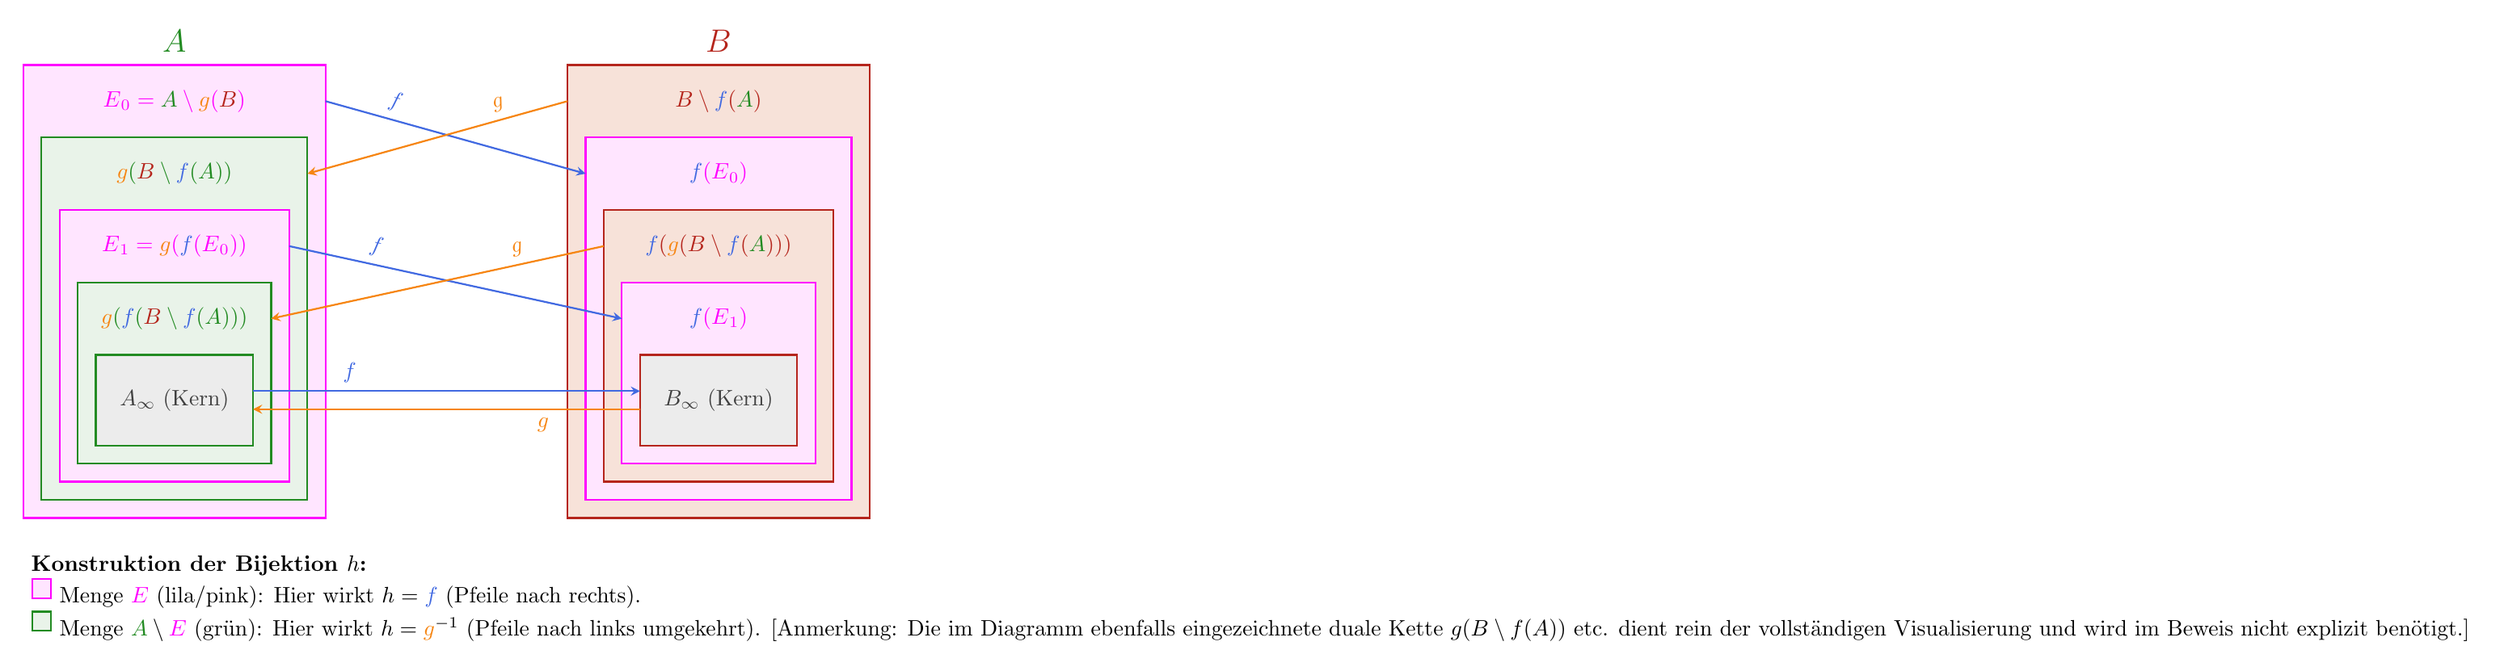
\begin{tikzpicture}[scale=0.95, >=stealth]
  
  \colorlet{colA}{ForestGreen}
  \colorlet{colB}{BrickRed}
  \colorlet{colE}{Fuchsia}
  \colorlet{colF}{RoyalBlue}
  \colorlet{colG}{BurntOrange}
  
  \colorlet{fillA}{ForestGreen!10}
  \colorlet{fillB}{BrickRed!10}
  \colorlet{fillE}{Fuchsia!10}
  \colorlet{fillCore}{gray!15}

  % Set A (Verschachtelungen)
  \filldraw[fill=fillE, draw=colE, thick] (0,0) rectangle (5,7.5);
  \filldraw[fill=fillA, draw=colA, thick] (0.3,0.3) rectangle (4.7,6.3);
  \filldraw[fill=fillE, draw=colE, thick] (0.6,0.6) rectangle (4.4,5.1);
  \filldraw[fill=fillA, draw=colA, thick] (0.9,0.9) rectangle (4.1,3.9);
  \filldraw[fill=fillCore, draw=colA, thick] (1.2,1.2) rectangle (3.8,2.7);

  \node[colA, font=\Large\bfseries] at (2.5, 7.9) {$\textcolor{ForestGreen}{A}$};
  \node[colE] at (2.5, 6.9) {$\textcolor{Fuchsia}{E}_0 = \textcolor{ForestGreen}{A} \setminus \textcolor{BurntOrange}{g}(\textcolor{BrickRed}{B})$};
  \node[colA] at (2.5, 5.7) {$\textcolor{BurntOrange}{g}(\textcolor{BrickRed}{B} \setminus \textcolor{RoyalBlue}{f}(\textcolor{ForestGreen}{A}))$};
  \node[colE] at (2.5, 4.5) {$\textcolor{Fuchsia}{E}_1 = \textcolor{BurntOrange}{g}(\textcolor{RoyalBlue}{f}(\textcolor{Fuchsia}{E}_0))$};
  \node[colA] at (2.5, 3.3) {$\textcolor{BurntOrange}{g}(\textcolor{RoyalBlue}{f}(\textcolor{BrickRed}{B} \setminus \textcolor{RoyalBlue}{f}(\textcolor{ForestGreen}{A})))$};
  \node[darkgray] at (2.5, 1.95) {$A_\infty$ (Kern)};

  % Set B (Verschachtelungen)
  \filldraw[fill=fillB, draw=colB, thick] (9,0) rectangle (14,7.5);
  \filldraw[fill=fillE, draw=colE, thick] (9.3,0.3) rectangle (13.7,6.3);
  \filldraw[fill=fillB, draw=colB, thick] (9.6,0.6) rectangle (13.4,5.1);
  \filldraw[fill=fillE, draw=colE, thick] (9.9,0.9) rectangle (13.1,3.9);
  \filldraw[fill=fillCore, draw=colB, thick] (10.2,1.2) rectangle (12.8,2.7);

  \node[colB, font=\Large\bfseries] at (11.5, 7.9) {$\textcolor{BrickRed}{B}$};
  \node[colB] at (11.5, 6.9) {$\textcolor{BrickRed}{B} \setminus \textcolor{RoyalBlue}{f}(\textcolor{ForestGreen}{A})$};
  \node[colE] at (11.5, 5.7) {$\textcolor{RoyalBlue}{f}(\textcolor{Fuchsia}{E}_0)$};
  \node[colB] at (11.5, 4.5) {$\textcolor{RoyalBlue}{f}(\textcolor{BurntOrange}{g}(\textcolor{BrickRed}{B} \setminus \textcolor{RoyalBlue}{f}(\textcolor{ForestGreen}{A})))$};
  \node[colE] at (11.5, 3.3) {$\textcolor{RoyalBlue}{f}(\textcolor{Fuchsia}{E}_1)$};
  \node[darkgray] at (11.5, 1.95) {$B_\infty$ (Kern)};

  % Pfeile für f (Blau) - pos=0.25 setzt das Label nah an A
  \draw[->, colF, thick] (5, 6.9) -- node[above, sloped, pos=0.25] {$\textcolor{RoyalBlue}{f}$} (9.3, 5.7);
  \draw[->, colF, thick] (4.4, 4.5) -- node[above, sloped, pos=0.25] {$\textcolor{RoyalBlue}{f}$} (9.9, 3.3);
  \draw[->, colF, thick] (3.8, 2.1) -- node[above, pos=0.25] {$\textcolor{RoyalBlue}{f}$} (10.2, 2.1);

  % Pfeile für g (Orange) - pos=0.25 setzt das Label nah an B (da der Pfeil von B nach A geht)
  \draw[->, colG, thick] (9, 6.9) -- node[above, sloped, pos=0.25] {$\textcolor{BurntOrange}{g}$} (4.7, 5.7);
  \draw[->, colG, thick] (9.6, 4.5) -- node[above, sloped, pos=0.25] {$\textcolor{BurntOrange}{g}$} (4.1, 3.3);
  \draw[->, colG, thick] (10.2, 1.8) -- node[below, pos=0.25] {$\textcolor{BurntOrange}{g}$} (3.8, 1.8);

  % Legende
  \node[align=left, anchor=north west] at (0, -0.5) {
    \textbf{Konstruktion der Bijektion $h$:}\\
    \tikz[baseline=-0.5ex] \filldraw[fill=fillE, draw=colE, thick] (0,0) rectangle (0.3,0.3); Menge $\textcolor{Fuchsia}{E}$ (lila/pink): Hier wirkt $h = \textcolor{RoyalBlue}{f}$ (Pfeile nach rechts).\\
    \tikz[baseline=-0.5ex] \filldraw[fill=fillA, draw=colA, thick] (0,0) rectangle (0.3,0.3); Menge $\textcolor{ForestGreen}{A} \setminus \textcolor{Fuchsia}{E}$ (grün): Hier wirkt $h = \textcolor{BurntOrange}{g}^{-1}$ (Pfeile nach links umgekehrt). \inlinemetanote{[Anmerkung: Die im Diagramm ebenfalls eingezeichnete duale Kette $g(B \setminus f(A))$ etc. dient rein der vollständigen Visualisierung und wird im Beweis nicht explizit benötigt.]}
  };
\end{tikzpicture}
\end{center}

\textbf{1. Wohldefiniertheit von $h$:} \\
Falls $x \notin \textcolor{Fuchsia}{E}$, so ist insbesondere $x \notin \textcolor{Fuchsia}{E}_0 = \textcolor{ForestGreen}{A} \setminus \textcolor{BurntOrange}{g}(\textcolor{BrickRed}{B})$. Daraus folgt $x \in \textcolor{BurntOrange}{g}(\textcolor{BrickRed}{B})$. Da $\textcolor{BurntOrange}{g}$ injektiv ist, existiert ein eindeutiges Urbild $\textcolor{BurntOrange}{g}^{-1}(x) \in \textcolor{BrickRed}{B}$. Somit ist $h$ wohldefiniert.

\textbf{2. Injektivität von $h$:} \\
Seien $x_1, x_2 \in \textcolor{ForestGreen}{A}$ mit $h(x_1) = h(x_2)$.
\begin{itemize}
    \item \textbf{Fall 1 ($x_1, x_2 \in \textcolor{Fuchsia}{E}$):} Es gilt $\textcolor{RoyalBlue}{f}(x_1) = \textcolor{RoyalBlue}{f}(x_2)$. Da $\textcolor{RoyalBlue}{f}$ injektiv ist, folgt daraus $x_1 = x_2$.
    \item \textbf{Fall 2 ($x_1, x_2 \notin \textcolor{Fuchsia}{E}$):} Es gilt $\textcolor{BurntOrange}{g}^{-1}(x_1) = \textcolor{BurntOrange}{g}^{-1}(x_2)$. Da $\textcolor{BurntOrange}{g}$ injektiv ist, folgt daraus $x_1 = x_2$.
    \item \textbf{Fall 3 (Mischfall):} Angenommen, $x_1 \in \textcolor{Fuchsia}{E}$ und $x_2 \notin \textcolor{Fuchsia}{E}$. Dann gilt $\textcolor{RoyalBlue}{f}(x_1) = \textcolor{BurntOrange}{g}^{-1}(x_2)$. Da $x_2 \notin \textcolor{Fuchsia}{E}$, liegt $x_2$ im Bild von $\textcolor{BurntOrange}{g}$, weshalb die Anwendung von $\textcolor{BurntOrange}{g}$ auf beide Seiten wohldefiniert ist und $\textcolor{BurntOrange}{g}(\textcolor{RoyalBlue}{f}(x_1)) = x_2$ liefert. Da $x_1 \in \textcolor{Fuchsia}{E}$, existiert ein $n \in \omega$ mit $x_1 \in \textcolor{Fuchsia}{E}_n$. Daraus ergibt sich $x_2 = \textcolor{BurntOrange}{g}(\textcolor{RoyalBlue}{f}(x_1)) \in \textcolor{Fuchsia}{E}_{n+1} \subseteq \textcolor{Fuchsia}{E}$, was im Widerspruch zu $x_2 \notin \textcolor{Fuchsia}{E}$ steht.
\end{itemize}
Somit ist $h$ injektiv.

\textbf{3. Surjektivität von $h$:} \\
Sei $y \in \textcolor{BrickRed}{B}$. Wir suchen ein $x \in \textcolor{ForestGreen}{A}$ mit $h(x) = y$.
\begin{itemize}
    \item \textbf{Fall 1 ($\textcolor{BurntOrange}{g}(y) \in \textcolor{Fuchsia}{E}$):} Dann existiert ein $n \in \omega$ mit $\textcolor{BurntOrange}{g}(y) \in \textcolor{Fuchsia}{E}_n$. Da $\textcolor{BurntOrange}{g}(y) \in \textcolor{BurntOrange}{g}(\textcolor{BrickRed}{B})$, kann $\textcolor{BurntOrange}{g}(y)$ nicht in $\textcolor{Fuchsia}{E}_0$ liegen, also ist $n \ge 1$. Es gilt $\textcolor{BurntOrange}{g}(y) \in \textcolor{Fuchsia}{E}_n = \textcolor{BurntOrange}{g}(\textcolor{RoyalBlue}{f}(\textcolor{Fuchsia}{E}_{n-1}))$. Da $\textcolor{BurntOrange}{g}$ injektiv ist, folgt $y = \textcolor{RoyalBlue}{f}(x)$ für ein $x \in \textcolor{Fuchsia}{E}_{n-1} \subseteq \textcolor{Fuchsia}{E}$. Für dieses $x$ gilt $h(x) = \textcolor{RoyalBlue}{f}(x) = y$.
    \item \textbf{Fall 2 ($\textcolor{BurntOrange}{g}(y) \notin \textcolor{Fuchsia}{E}$):} Wir wählen $x := \textcolor{BurntOrange}{g}(y) \notin \textcolor{Fuchsia}{E}$. Dann gilt $h(x) = \textcolor{BurntOrange}{g}^{-1}(x) = \textcolor{BurntOrange}{g}^{-1}(\textcolor{BurntOrange}{g}(y)) = y$.
\end{itemize}
Somit ist $h$ surjektiv und folglich eine Bijektion. Es gilt $|\textcolor{ForestGreen}{A}| = |\textcolor{BrickRed}{B}|$.
\end{short-proof}
\end{math-stroke}

\begin{ai-note}[Zur Notation der Umkehrfunktion $g^{-1}$]
Da die Abbildung $g \colon B \to A$ im Allgemeinen nicht surjektiv ist, existiert die globale Umkehrfunktion $g^{-1}$ streng genommen nicht auf der gesamten Menge $A$. Wenn wir im Beweis $g^{-1}(x)$ schreiben, ist damit präzise das eindeutige Element $y \in B$ gemeint, für das $g(y) = x$ gilt. Dieses $y$ existiert nachweislich für alle $x \notin E$, da diese Elemente konstruktionsbedingt im Bild von $g$ liegen, und es ist eindeutig, da $g$ injektiv ist.
\end{ai-note}

\begin{didactic-insight}[Die Eleganz des Cantor-Bernstein-Schröder-Theorems]
Der Beweis des Cantor-Bernstein-Schröder-Theorems ist ein klassisches Beispiel für ein faszinierend konstruktives Verfahren in der axiomatischen Mengenlehre. Im Gegensatz zu vielen anderen fundamentalen Sätzen über unendliche Mächtigkeiten kommt dieser Beweis komplett ohne das Auswahlaxiom (Axiom of Choice) aus und ist somit bereits in der Standard-Zermelo-Fraenkel-Mengenlehre (ZF) uneingeschränkt gültig. 

Anstatt eine unendliche Auswahl zu treffen oder ein Wohlordnungsprinzip anzunehmen, wird die gesuchte Bijektion $h$ explizit, deterministisch und schrittweise durch die Mengenfolge $E_n$ konstruiert (im Englischen oft auch als \qt{Ping-Pong-Argument} bezeichnet).

Die Grafik veranschaulicht die Genialität dieses konstruktiven Ansatzes: Die Funktion $h$ partitioniert die Menge $\textcolor{ForestGreen}{A}$ geschickt in verschachtelte Ringe von Vor- und Nachbildern, um lokale Teilstücke von Bijektionen nahtlos zusammenzuflicken:
\begin{align*}
  \textcolor{ForestGreen}{A} &= \textcolor{Fuchsia}{E} \;\dot{\cup}\; (\textcolor{ForestGreen}{A} \setminus \textcolor{Fuchsia}{E}) \\
  \textcolor{BrickRed}{B} &= \textcolor{RoyalBlue}{f}(\textcolor{Fuchsia}{E}) \;\dot{\cup}\; (\textcolor{BrickRed}{B} \setminus \textcolor{RoyalBlue}{f}(\textcolor{Fuchsia}{E}))
\end{align*}
Auf der lila/pinken Teilmenge $\textcolor{Fuchsia}{E}$ verwenden wir die direkte \qt{Vorwärtsabbildung} $\textcolor{RoyalBlue}{f}$, während wir auf dem grünen Komplement $\textcolor{ForestGreen}{A} \setminus \textcolor{Fuchsia}{E}$ die Umkehrung der \qt{Rückwärtsabbildung} $\textcolor{BurntOrange}{g}^{-1}$ nutzen, um den Rest der Mengen perfekt auszufüllen.
\end{didactic-insight}

\section{Gleichmächtigkeit von \texorpdfstring{$\mathbb{R}$}{R} und der Potenzmenge von \texorpdfstring{$\omega$}{omega}}

\subsection{Beispiel: Abzählbarkeit der rationalen Zahlen}

\begin{spoken-clean}[00:30:49 - 00:32:41]
Schauen wir uns diesbezüglich noch ein paar Beispiele an. Schauen wir uns zum Beispiel ein klassisches Beispiel an, das Sie wahrscheinlich auch schon kennen: dass die rationalen Zahlen gleichmächtig zu den natürlichen Zahlen --- also zu den positiven ganzen Zahlen --- sind.

Für den Beweis müssen wir eine Injektion von der einen in die andere Richtung und umgekehrt konstruieren. Das Erste, nämlich dass $|\omega| \le |\mathbb{Q}|$ gilt, ist klar. Wir können einfach die Abbildung von $\omega$ nach $\mathbb{Q}$ betrachten, die ein Element $n$ auf $n$ geteilt durch $1$ abbildet. Das ist offensichtlich injektiv.
\end{spoken-clean}

\begin{math-stroke}[Injektion von den natürlichen in die rationalen Zahlen]
\begin{proposition}\label[proposition]{prop:omega-le-q}
Es gilt:
\[
|\omega| \le |\mathbb{Q}|
\]
\end{proposition}
\begin{short-proof}[Beweis von \cref{prop:omega-le-q}]
Wir definieren die kanonische Einbettung $i \colon \omega \to \mathbb{Q}$ durch:
\[
i(n) := \frac{n}{1}
\]
Da für alle $n, m \in \omega$ gilt:
\[
i(n) = i(m) \implies \frac{n}{1} = \frac{m}{1} \implies n = m
\]
ist diese Abbildung $i$ eine Injektion. Somit gilt $|\omega| \le |\mathbb{Q}|$.
\end{short-proof}
\end{math-stroke}

\begin{spoken-clean}[00:32:41 - 00:33:40]
Das heißt, was wir jetzt noch zeigen müssen, ist eine Injektion von $\mathbb{Q}$ nach $\omega$.

Dazu betrachten wir einfach die Abbildung von $\mathbb{Q}$ nach $\omega$, gegeben durch $f\left(\frac{p}{q}\right)$, wobei wir annehmen, dass $p$ und $q$ teilerfremd sind. Wir definieren: Das soll $0$ sein, falls $p$ gleich $0$ ist. Und wir sagen, das soll einfach $2^p \cdot 3^q$ sein, falls $p$ und $q$ beide größer als $0$ sind. Und es soll $2^{|p|} \cdot 5^q$ sein, falls $p$ kleiner als $0$ und $q$ größer als $0$ ist. In beiden Fällen nehmen wir an, dass der größte gemeinsame Teiler von $|p|$ und $q$ gleich $1$ ist.
\end{spoken-clean}

\begin{student-interaction}[Korrektur der Abbildungsrichtung]
Äh, $\mathbb{Q}$ nach $\omega$, danke schön. Danke, natürlich $\mathbb{Q}$ nach $\omega$.
\end{student-interaction}

\begin{spoken-clean}[00:33:40 - 00:34:04]
Danke, natürlich von $\mathbb{Q}$ nach $\omega$. Ansonsten hätten wir ja wieder die Abbildung von $\omega$ nach $\mathbb{Q}$, die wir oben schon hatten. Genau.
\end{spoken-clean}

\begin{spoken-clean}[00:34:04 - 00:35:33]
Das werden wir noch genauer betrachten, wenn wir uns ein bisschen mit elementarer Zahlentheorie beschäftigen. Aber vielleicht wissen Sie schon aus der Schule oder aus einer anderen Vorlesung, dass es für jede natürliche Zahl eine eindeutige Faktorisierung in Primzahlen gibt. Das heißt, wenn $p$ und $q$ verschieden sind, sind diese Zahlen hier alle verschieden. Und sie sind wiederum alle verschieden von den anderen, weil wir hier eine andere Primfaktorzerlegung haben.

Und genau, wir können ja auch immer annehmen, dass $p$ und $q$ teilerfremd sind. Das heißt, das ist tatsächlich eine Injektion. Okay, ich schreibe jetzt einfach: \qt{ist injektiv} (gemäß der Eindeutigkeit der Primfaktorzerlegung). Aber wir setzen hier natürlich die eindeutige Primfaktorzerlegung voraus, die wir formal noch nicht bewiesen haben.
\end{spoken-clean}

\begin{math-stroke}[Injektion von den rationalen in die natürlichen Zahlen]
\begin{proposition}[Abzählbarkeit der rationalen Zahlen]\label[proposition]{prop:q-le-omega}
Es gilt:
\[
|\mathbb{Q}| \le |\omega|
\]
\end{proposition}
\begin{short-proof}[Beweis von \cref{prop:q-le-omega}]
Jede rationale Zahl $x \in \mathbb{Q} \setminus \{0\}$ lässt sich eindeutig als gekürzter Bruch darstellen:
\[
x = \frac{p}{q} \quad \text{mit } p \in \mathbb{Z} \setminus \{0\}, \ q \in \omega \setminus \{0\} \quad \text{und} \quad \operatorname{ggT}(|p|, q) = 1
\]
Wir definieren die Abbildung $f \colon \mathbb{Q} \to \omega$ durch:
\begin{equation}\label{eq:prime-injection}
f\left(\frac{p}{q}\right) := \begin{cases}
0 & \text{falls } p = 0 \\
2^p \cdot 3^q & \text{falls } p > 0 \\
2^{|p|} \cdot 5^q & \text{falls } p < 0
\end{cases}
\end{equation}
Die Injektivität dieser Abbildung folgt direkt aus dem \newterm{Fundamentalsatz der Arithmetik} (der Eindeutigkeit der Primfaktorzerlegung in $\mathbb{N}$):
Da die Primfaktoren $2, 3$ und $5$ paarweise verschieden sind, haben Bilder von positiven Brüchen, negativen Brüchen und der Null disjunkte Primfaktorzerlegungen. Da zudem $\operatorname{ggT}(|p|, q) = 1$ gilt, ist die Zuordnung eindeutig. Somit ist $f$ injektiv, und es gilt $|\mathbb{Q}| \le |\omega|$.
\end{short-proof}

\begin{corollary}[Abzählbarkeit der rationalen Zahlen]\label[corollary]{cor:q-countable}
Es gilt:
\[
|\mathbb{Q}| = |\omega|
\]
\end{corollary}
\begin{short-proof}[Beweis von \cref{cor:q-countable}]
Die Behauptung folgt unmittelbar aus Proposition \ref{prop:omega-le-q} ($|\omega| \le |\mathbb{Q}|$), Proposition \ref{prop:q-le-omega} ($|\mathbb{Q}| \le |\omega|$) und dem Cantor-Bernstein-Schröder-Theorem (Theorem \ref{thm:cantor-bernstein-schroeder}).
\end{short-proof}
\end{math-stroke}

\subsection{Gleichmächtigkeit der Reellen und der Potenzmenge von \texorpdfstring{$\omega$}{omega}}

\begin{spoken-clean}[00:35:33 - 00:37:51]
Gut, und dann noch ein weiteres Beispiel, das Sie vielleicht auch schon in den Übungen angeschaut haben, ohne diesen Satz zur Verfügung zu haben: das ist die Mächtigkeit der reellen Zahlen. Diese Proposition besagt nun, dass die reellen Zahlen dieselbe Kardinalität wie die Potenzmenge von $\omega$ besitzen. Das haben Sie in den Übungen bereits besprochen und gelöst. Ich kann es aber gerne nochmals kurz erklären.

Der Beweis läuft wie folgt: Wir wissen, dass die Mächtigkeit der reellen Zahlen kleiner gleich der Mächtigkeit der Potenzmenge von $\omega$ ist. Weshalb ist das der Fall? Nun, das kommt darauf an, wie wir die reellen Zahlen definieren. Wir haben sie ja über Dedekind-Schnitte definiert, und Dedekind-Schnitte sind per Definition Teilmengen der rationalen Zahlen. Und wir haben gerade gesehen, dass die rationalen Zahlen bei uns bijektiv zu den natürlichen Zahlen sind; folglich sind auch ihre Potenzmengen bijektiv zueinander.

Da die reellen Zahlen eine Teilmenge der Potenzmenge von $\mathbb{Q}$ sind, ist die Kardinalität von $\mathbb{R}$ insbesondere kleiner gleich der Kardinalität von $\mathcal{P}(\mathbb{Q})$. Und die Potenzmenge von $\mathbb{Q}$ hat wiederum dieselbe Kardinalität wie die Potenzmenge von $\omega$, da wir eine Bijektion zwischen $\omega$ und $\mathbb{Q}$ haben, die natürlich eine Bijektion zwischen den Potenzmengen induziert. Somit wissen wir per Konstruktion aus den Dedekind-Schnitten, dass die Kardinalität von $\mathbb{R}$ nicht größer sein kann als diejenige von $\mathcal{P}(\omega)$. An dieser Stelle nutzen wir also die Definition von $\mathbb{R}$ über Dedekind-Schnitte.
\end{spoken-clean}

\begin{math-stroke}[Abschätzung der reellen Zahlen nach oben]
\begin{proposition}\label[proposition]{prop:r-le-p-omega}
Es gilt:
\[
|\mathbb{R}| \le |\mathcal{P}(\omega)|
\]
\end{proposition}
\begin{short-proof}[Beweis von \cref{prop:r-le-p-omega}]
Wir haben die reellen Zahlen $\mathbb{R}$ über Dedekindsche Schnitte als Teilmenge der Potenzmenge der rationalen Zahlen definiert (Definition \ref{def:reelle-zahlen}):
\[
\mathbb{R} \subseteq \mathcal{P}(\mathbb{Q}) \implies |\mathbb{R}| \le |\mathcal{P}(\mathbb{Q})|
\]
Da nach Korollar \ref{cor:q-countable} eine Bijektion $g \colon \mathbb{Q} \to \omega$ existiert, induziert diese eine kanonische Bijektion zwischen den Potenzmengen:
\[
G \colon \mathcal{P}(\mathbb{Q}) \to \mathcal{P}(\omega), \quad A \mapsto \{ g(a) \mid a \in A \}
\]
Daraus folgt $|\mathcal{P}(\mathbb{Q})| = |\mathcal{P}(\omega)|$. Zusammen mit der obigen Inklusion erhalten wir:
\[
|\mathbb{R}| \le |\mathcal{P}(\omega)|
\]
\end{short-proof}
\end{math-stroke}

\begin{spoken-clean}[00:37:51 - 00:40:36]
Umgekehrt wollen wir zeigen, dass eine Injektion von der Potenzmenge von $\omega$ nach $\mathbb{R}$ existiert.

Dazu betrachten wir einfach die Abbildung $f \colon \mathcal{P}(\omega) \to \mathbb{R}$, gegeben durch eine summe: Wir schicken eine Teilmenge $X$ auf die Summe über alle $n \in X$ von $3^{-n-1}$ --- ob wir $3^{-n}$ oder $3^{-n-1}$ nehmen, ist im Prinzip egal. Das liefert uns eine Injektion. Wir haben also eine Injektion von der Potenzmenge von $\omega$ nach $\mathbb{R}$.

Dass diese Abbildung tatsächlich injektiv ist, ist eine sehr schöne Übung. Und da wir nun Injektionen in beide Richtungen haben, liefert uns der Satz von Cantor-Bernstein-Schröder eine Bijektion.
\end{spoken-clean}

\begin{math-stroke}[Abschätzung der reellen Zahlen nach unten]
\begin{proposition}\label[proposition]{prop:p-omega-le-r}
Es gilt:
\[
|\mathcal{P}(\omega)| \le |\mathbb{R}|
\]
\end{proposition}
\begin{short-proof}[Beweis von \cref{prop:p-omega-le-r}]
Wir konstruieren eine explizite Injektion $f \colon \mathcal{P}(\omega) \to \mathbb{R}$. Für jede Teilmenge $X \subseteq \omega$ definieren wir das Bild $f(X)$ über eine unendliche Reihe:
\begin{equation}\label{eq:ternary-injection}
f(X) := \sum_{n \in X} \frac{1}{3^{n+1}}
\end{equation}
Da für alle $n \in \omega$ der Summand $\frac{1}{3^{n+1}} > 0$ is, konvergiert diese Reihe für jede Teilmenge $X$ absolut gegen eine reelle Zahl im Intervall $[0, \frac{1}{2}]$, da:
\[
\sum_{n \in X} \frac{1}{3^{n+1}} \le \sum_{n=0}^\infty \frac{1}{3^{n+1}} = \frac{1}{3} \cdot \frac{1}{1 - 1/3} = \frac{1}{2}
\]
Die Injektivität von $f$ folgt aus den Eigenschaften der triadischen Entwicklung (Basis 3): Da wir als Koeffizienten der Entwicklung nur $0$ (falls $n \notin X$) und $1$ (falls $n \in X$) verwenden, vermeiden wir das Problem der mehrdeutigen Darstellungen (wie im Dezimalsystem $0{,}1999\dots = 0{,}2000\dots$). Eine triadische Zahl mit Koeffizienten aus $\{0, 1\}$ ist eindeutig bestimmt. Somit ist $f$ injektiv, und es gilt $|\mathcal{P}(\omega)| \le |\mathbb{R}|$.
\end{short-proof}

\begin{theorem}[Gleichmächtigkeit des Kontinuums]\label[theorem]{thm:r-equals-p-omega}
Es gilt:
\[
|\mathbb{R}| = |\mathcal{P}(\omega)|
\]
\end{theorem}
\begin{short-proof}[Beweis von \cref{thm:r-equals-p-omega}]
Die Behauptung folgt direkt aus Proposition \ref{prop:r-le-p-omega} ($|\mathbb{R}| \le |\mathcal{P}(\omega)|$), Proposition \ref{prop:p-omega-le-r} ($|\mathcal{P}(\omega)| \le |\mathbb{R}|$) und dem Cantor-Bernstein-Schröder-Theorem (Theorem \ref{thm:cantor-bernstein-schroeder}).
\end{short-proof}
\end{math-stroke}

\section{Der Satz von Cantor}

\begin{spoken-clean}[00:40:36 - 00:42:42]
Ja, und das ist in der Praxis natürlich äußerst praktisch, um zu zeigen, dass zwei Mengen gleichmächtig sind. Wie Sie wissen, ist es manchmal recht mühsam, eine explizite Bijektion direkt zu konstruieren; es ist viel einfacher, stattdessen Injektionen zu finden.

Schauen wir uns diesbezüglich noch ein paar Beispiele an. Nun, als Nächstes betrachten wir den Satz von Cantor. Ich schreibe ihn noch schnell an die Tafel, dann können wir ihn nach der Pause direkt beweisen. Den hat Cantor tatsächlich auch schon bewiesen, und er besagt, dass für jede Menge $M$ gilt, dass die Mächtigkeit von $M$ strikt kleiner ist als die Mächtigkeit ihrer Potenzmenge. Wenn wir also die Potenzmenge einer Menge $M$ betrachten, dann hat diese immer eine echt größere Mächtigkeit als $M$ selbst.

Genau, das werden wir nach der Pause beweisen. Danach werden wir die Kardinalzahlen formal definieren --- das läuft ganz ähnlich wie bei den Ordinalzahlen. Gut, machen wir eine schöne Pause!
\end{spoken-clean}

\begin{math-stroke}
\begin{theorem}[Satz von Cantor]\label[theorem]{thm:cantor}
Für jede Menge $M$ gilt:
\[
|M| < |\mathcal{P}(M)|
\]
\end{theorem}
\end{math-stroke}

\begin{lecture-break}[Pause: 11 Minuten]
\end{lecture-break}

\section{Kardinalzahlen und ihre Arithmetik}

\begin{spoken-clean}[00:54:02 - 00:54:37]
... Menge, und wenn das keine Menge wäre, könnten wir keine Durchschnitte über Objekte bilden, die keine Mengen sind. Aber man kann zeigen, dass dies tatsächlich eine Menge ist. Das sind also wohldefinierte Mengen für alle $M$.
\end{spoken-clean}

\subsection{Definition der Kardinalzahlen}

\begin{spoken-clean}[00:54:37 - 00:55:45]
Gut, und wir definieren jetzt einfach: Eine Kardinalzahl ist eine Ordinalzahl, die nicht gleichmächtig zu einer kleineren Ordinalzahl ist. Das heißt, wir betrachten die Ordinalzahlen, von denen manche gleichmächtig zu kleineren Ordinalzahlen sind. Zum Beispiel ist $\omega + 1$ gleichmächtig zu $\omega$. Das bedeutet, $\omega + 1$ ist keine Kardinalzahl.

Aber $\omega$ ist eine Kardinalzahl, weil jede kleinere Ordinalzahl endlich ist, während $\omega$ unendlich ist; folglich kann $\omega$ nicht gleichmächtig zu einer kleineren Ordinalzahl sein. Auch alle endlichen Ordinalzahlen --- also die natürlichen Zahlen --- sind Kardinalzahlen, weil keine natürliche Zahl gleichmächtig zu einer kleineren natürlichen Zahl ist. Das ist genau das, was wir uns jetzt überlegen wollen.
\end{spoken-clean}

\begin{math-stroke}
\begin{definition}[Kardinalzahl]\label[definition]{def:kardinalzahl}
Eine Ordinalzahl $\kappa \in \Omega$ heißt \newterm{Kardinalzahl}, falls für alle Ordinalzahlen $\alpha < \kappa$ gilt \inlinemetanote{[Anmerkung: Da wir bereits $|\alpha| \le |\kappa|$ durch die Inklusion $\alpha \subseteq \kappa$ wissen, ist die Bedingung $|\alpha| < |\kappa|$ äquivalent zu $|\alpha| \neq |\kappa|$, was der gesprochenen Intuition entspricht]}:
\begin{equation}\label{eq:kardinalzahl-def}
|\alpha| < |\kappa|
\end{equation}
\end{definition}
\end{math-stroke}

\subsection{Kardinalität in ZFC}

\begin{spoken-clean}[00:55:45 - 00:57:32]
Wie definieren wir nun die Kardinalität einer beliebigen Menge? In der Zermelo-Fraenkel-Mengenlehre mit Auswahlaxiom haben wir das Wohlordnungsprinzip zur Verfügung. Das Wohlordnungsprinzip besagt, dass jede Menge wohlgeordnet werden kann. Und wir haben bereits gesehen, dass jede wohlgeordnete Menge isomorph zu einer eindeutigen Ordinalzahl ist. Das heißt, für jede Menge $M$ existiert eine Ordinalzahl $\alpha$, sodass $M$ gleichmächtig zu $\alpha$ ist.

Es kann natürlich viele solche Ordinalzahlen geben. Wenn $M$ beispielsweise abzählbar unendlich ist, dann ist $M$ gleichmächtig zu $\omega$, zu $\omega + 1$, zu $\omega + 2$ und so weiter. Da die Ordinalzahlen jedoch wohlgeordnet sind, gibt es eine eindeutige kleinste solche Ordinalzahl. Und genau diese kleinste Ordinalzahl definieren wir als die Kardinalität von $M$. Das ist die Standarddefinition der Kardinalität in ZFC.
\end{spoken-clean}

\begin{math-stroke}[Kardinalität unter dem Wohlordnungsprinzip]
Gemäß dem Wohlordnungsprinzip (\textbf{WOP}, \cref{thm:wohlordnungsprinzip}) existiert für jede Menge $M$ eine Ordinalzahl $\alpha \in \Omega$ mit $|M| = |\alpha|$.

\begin{definition}[Kardinalität einer Menge]\label[definition]{def:kardinalitaet-menge}
Die \newterm{Kardinalität} (oder Mächtigkeit) $|M|$ einer Menge $M$ ist die kleinste Ordinalzahl $\alpha$, die gleichmächtig zu $M$ ist:
\begin{equation}\label{eq:kardinalitaet-def}
|M| := \min \{ \alpha \in \Omega \mid |\alpha| = |M| \}
\end{equation}
\end{definition}

\begin{explanation-of-steps}[Warum diese Definition nicht zirkulär ist]
Auf den ersten Blick scheint $|M|$ hier durch sich selbst definiert zu werden. Das ist nicht der Fall: Der Ausdruck \qt{$|\alpha| = |M|$} ist nach \cref{def:gleichmaechtigkeit} \emph{keine} Gleichung zwischen zwei bereits definierten Objekten, sondern eine einzige, primitive zweistellige Relation --- nämlich \qt{es gibt eine Bijektion zwischen $\alpha$ und $M$}. Erst diese Definition erklärt das Symbol $|M|$ als eigenständiges Objekt (eine Ordinalzahl). Dass das Minimum existiert, folgt daraus, dass die Ordinalzahlen wohlgeordnet sind (\cref{thm:eigenschaften-omega} \textbf{(5)}), und dass die Menge überhaupt nicht leer ist, garantiert das Wohlordnungsprinzip.
\end{explanation-of-steps}
\end{math-stroke}

\subsection{Eigenschaften von Kardinalzahlen}

\begin{spoken-clean}[00:57:32 - 00:59:25]
Bemerkung: Wenn $\kappa$ eine Kardinalzahl ist, was ist dann die Kardinalität von $\kappa$? Das ist natürlich $\kappa$ selbst, weil $\kappa$ ja die kleinste Ordinalzahl ist, die gleichmächtig zu $\kappa$ ist. Für jede Kardinalzahl $\kappa$ gilt also $|\kappa| = \kappa$. Das ist eine sehr nützliche Eigenschaft.

Wir können auch zeigen, dass jede unendliche Kardinalzahl eine Limes-Ordinalzahl ist \inlinemetanote{[Anmerkung: Denn andernfalls wäre sie von der Form $\kappa = \alpha + 1$, und für unendliche Mengen gilt $|\alpha + 1| = |\alpha|$, was der Eigenschaft $|\alpha| < |\kappa|$ einer Kardinalzahl widerspricht]} --- das gilt natürlich nicht für die endlichen Kardinalzahlen, aber für unendliche Kardinalzahlen gilt das immer. Und wir schreiben für diese unendlichen Kardinalzahlen oft $\aleph_\alpha$ oder $\omega_\alpha$.
\end{spoken-clean}

\begin{math-stroke}[Eigenschaften von Kardinalzahlen]
\begin{remark}[Kardinalität von Kardinalzahlen]\label[remark]{rem:kardinalitaet-kardinalzahl}
Falls $\kappa$ eine Kardinalzahl ist, so gilt:
\[
|\kappa| = \kappa
\]
\end{remark}

\begin{notation}[Aleph-Notation]\label[notation]{not:aleph-notation}
Wir bezeichnen die $\alpha$-te unendliche Kardinalzahl mit $\omega_\alpha$ oder mit dem hebräischen Buchstaben Aleph als:
\[
\aleph_\alpha := \omega_\alpha
\]
Insbesondere ist $\aleph_0 = \omega_0 = \omega$ die kleinste unendliche Kardinalzahl.
\end{notation}
\end{math-stroke}

\subsection{Beweis des Satzes von Cantor}

\begin{spoken-clean}[00:59:25 - 01:00:55]
Kommen wir nun zum Satz von Cantor. Den haben wir vor der Pause schon angeschrieben, aber jetzt wollen wir ihn formal beweisen. Der Satz besagt: Für jede Menge $M$ gilt, dass die Mächtigkeit von $M$ strikt kleiner ist als die Mächtigkeit der Potenzmenge von $M$. Das heißt: $|M| < |\mathcal{P}(M)|$.

Wir beweisen das zuerst für den Fall, dass $M$ die leere Menge ist. Das ist ganz einfach: Wenn $M$ leer ist, dann ist die Potenzmenge von $M$ die Menge, die nur die leere Menge enthält. Das heißt, die Potenzmenge hat genau ein Element, während $M$ null Elemente besitzt. Da $0 < 1$ gilt, stimmt die Behauptung in diesem Fall. Für den allgemeinen Beweis nehmen wir nun an, dass $M$ nicht leer ist.
\end{spoken-clean}

\begin{math-stroke}
\begin{short-proof}[Beweis von \cref{thm:cantor} für $M = \emptyset$]
Falls $M = \emptyset$, so gilt:
\[
\mathcal{P}(\emptyset) = \{\emptyset\} \implies |\mathcal{P}(\emptyset)| = 1 > 0 = |\emptyset|
\]
Somit gilt die Behauptung trivialerweise für die leere Menge.
\end{short-proof}
\end{math-stroke}

\begin{spoken-clean}[01:00:55 - 01:02:29]
Um zu zeigen, dass $|M| < |\mathcal{P}(M)|$ für eine nichtleere Menge $M$ gilt, müssen wir zwei Dinge nachweisen. Erstens, dass $|M| \le |\mathcal{P}(M)|$ gilt. Das heißt, es muss eine Injektion von $M$ in die Potenzmenge von $M$ existieren. Das ist sehr einfach: Wir bilden jedes Element $x \in M$ auf die Einermenge $\{x\}$ ab. Das ist offensichtlich eine injektive Abbildung.

Zweitens müssen wir zeigen, dass keine Bijektion existieren kann. Das bedeutet, wir müssen zeigen, dass jede beliebige Abbildung $g$ von $M$ in die Potenzmenge von $M$ nicht surjektiv sein kann. Wenn uns dieser Nachweis gelingt, sind wir fertig.
\end{spoken-clean}

\begin{math-stroke}[Injektivität und Nicht-Surjektivität]
Sei $M \neq \emptyset$.
\begin{itemize}
    \item \textbf{Injektion:} Die Abbildung $f \colon M \to \mathcal{P}(M), x \mapsto \{x\}$ ist injektiv, woraus $|M| \le |\mathcal{P}(M)|$ folgt.
    \item \textbf{Nicht-Surjektivität:} Sei $g \colon M \to \mathcal{P}(M)$ eine beliebige Abbildung. Wir zeigen, dass $g$ nicht surjektiv sein kann.
\end{itemize}
\end{math-stroke}

\begin{spoken-clean}[01:02:29 - 01:03:23]
Dazu definieren wir die Menge $\Gamma$. Das ist die Menge aller Elemente $x \in M$, die nicht in ihrem eigenen Bild unter $g$ liegen. Also: $\Gamma = \{ x \in M \mid x \notin g(x) \}$. Da $\Gamma$ eine Teilmenge von $M$ ist, ist $\Gamma$ ein Element der Potenzmenge von $M$.

Wäre $g$ nun surjektiv, dann müsste ein Element $x_0 \in M$ existieren mit $g(x_0) = \Gamma$. Wir fragen uns nun: Liegt dieses $x_0$ in $\Gamma$ oder nicht? Wenn $x_0 \in \Gamma$ gilt, dann folgt nach Definition von $\Gamma$, dass $x_0 \notin g(x_0) = \Gamma$ ist --- ein Widerspruch. Wenn andererseits $x_0 \notin \Gamma$ gilt, dann folgt nach Definition von $\Gamma$, dass $x_0 \in g(x_0) = \Gamma$ sein muss --- ebenfalls ein Widerspruch. Das bedeutet, ein solches Element $x_0$ kann nicht existieren, und somit ist $g$ nicht surjektiv.
\end{spoken-clean}

\begin{math-stroke}[Beweis der Nicht-Surjektivität]
Wir definieren die Russell-artige Menge:
\[
\Gamma := \{ x \in M \mid x \notin g(x) \} \in \mathcal{P}(M)
\]
Angenommen, $g$ wäre surjektiv. Dann existiert ein Urbild $x_0 \in M$ mit:
\[
g(x_0) = \Gamma
\]
Wir untersuchen die Zugehörigkeit von $x_0$ zu $\Gamma$:
\[
x_0 \in \Gamma \iff x_0 \notin g(x_0) \iff x_0 \notin \Gamma
\]
Dies ist ein logischer Widerspruch. Folglich existiert kein solches $x_0$, und $\Gamma$ liegt nicht im Bild von $g$. Somit ist $g$ nicht surjektiv, was den Beweis abschließt.
\end{math-stroke}

\subsection{Die Kontinuumshypothese}

\begin{spoken-clean}[01:03:23 - 01:05:20]
Kommen wir nun zu einem der berühmtesten Themen der Mengenlehre: der Kontinuumshypothese. Wir haben gesehen, dass die Mächtigkeit von $\omega$ strikt kleiner ist als die Mächtigkeit der Potenzmenge von $\omega$. Und wir wissen bereits, dass die Potenzmenge von $\omega$ gleichmächtig zu den reellen Zahlen $\mathbb{R}$ ist. Das heißt: $|\omega| < |\mathcal{P}(\omega)| = |\mathbb{R}| = 2^\omega$. Wir bezeichnen die Mächtigkeit der reellen Zahlen oft mit $\mathfrak{c}$ oder mit $2^{\aleph_0}$.
\end{spoken-clean}

\begin{spoken-clean}[01:05:20 - 01:07:21]
Da $\aleph_0$ die kleinste unendliche Kardinalzahl ist, ist die nächstgrößere unendliche Kardinalzahl $\aleph_1$. Die Kontinuumshypothese besagt nun, dass es keine Kardinalzahl strikt zwischen $\aleph_0$ und $2^{\aleph_0}$ gibt. Das heißt: $2^{\aleph_0} = \aleph_1$. Das war eines der berühmten Hilbert'schen Probleme, und im 20. Jahrhundert wurde bewiesen, dass diese Aussage unabhängig von den ZFC-Axiomen ist. Gödel hat gezeigt, dass man sie nicht widerlegen kann, und Cohen hat bewiesen, dass man sie nicht beweisen kann.
\end{spoken-clean}

\begin{math-stroke}
Wechselbeziehung zwischen abzählbaren und überabzählbaren Mengen:
\[
|\omega| < |\mathcal{P}(\omega)| = |\mathbb{R}| = 2^{\aleph_0} =: \mathfrak{c}
\]

\begin{definition}[Kontinuumshypothese]\label[definition]{def:kontinuumshypothese}
Die \newterm{Kontinuumshypothese} (\textbf{CH} -- Continuum Hypothesis) besagt, dass keine Kardinalzahl strikt zwischen $\aleph_0$ und $2^{\aleph_0}$ existiert:
\begin{equation}\label{eq:ch}
\aleph_1 = 2^{\aleph_0} = \mathfrak{c}
\end{equation}
\end{definition}

\begin{explanation-of-steps}[Unabhängigkeit von ZFC]
Die Kontinuumshypothese ist unabhängig von den Axiomen der Zermelo-Fraenkel-Mengenlehre mit Auswahlaxiom ($\text{ZFC}$):
\begin{itemize}
    \item \textbf{Kurt Gödel (1938):} Zeigte die relative Konsistenz von $\text{ZFC} + \text{CH}$ (mittels des konstruierbaren Universums $L$). $\text{CH}$ kann in $\text{ZFC}$ nicht widerlegt werden.
    \item \textbf{Paul Cohen (1963):} Zeigte die relative Konsistenz von $\text{ZFC} + \neg\text{CH}$ (mittels der Methode des Forcings). $\text{CH}$ kann in $\text{ZFC}$ nicht bewiesen werden.
\end{itemize}
\end{explanation-of-steps}
\end{math-stroke}

\subsection{Kardinalzahlarithmetik}

\begin{spoken-clean}[01:07:21 - 01:09:45]
Kommen wir nun zur Kardinalzahlarithmetik. Wir wollen definieren, wie man Kardinalzahlen addiert, multipliziert und potenziert. Das unterscheidet sich ein wenig von den Ordinalzahlen: Bei den Ordinalzahlen haben wir diese Operationen über die Ordnung definiert, aber bei den Kardinalzahlen definieren wir sie über die Mächtigkeiten von Mengen.
\end{spoken-clean}

\begin{spoken-clean}[01:09:45 - 01:12:09]
Seien $\kappa$ und $\lambda$ zwei Kardinalzahlen. Wir definieren die Summe $\kappa + \lambda$ als die Kardinalität der disjunkten Vereinigung zweier Mengen mit diesen Mächtigkeiten. Um das formal präzise zu machen, betrachten wir einfach die Mengen $\kappa \times \{0\}$ und $\lambda \times \{1\}$. Diese beiden Mengen sind offensichtlich disjunkt und haben die Mächtigkeiten $\kappa$ beziehungsweise $\lambda$. Die Summe ist dann definiert als die Kardinalität der Vereinigung dieser beiden Mengen. Das ist die formale Definition der Addition für Kardinalzahlen.
\end{spoken-clean}

\begin{math-stroke}
\begin{definition}[Addition von Kardinalzahlen]\label[definition]{def:kardinalzahl-addition}
Seien $\kappa$ und $\lambda$ Kardinalzahlen. Wir definieren ihre Summe als die Kardinalität der disjunkten Vereinigung:
\begin{equation}\label{eq:kardinalzahl-addition}
\kappa + \lambda := \bigl| (\kappa \times \{0\}) \cup (\lambda \times \{1\}) \bigr|
\end{equation}
\end{definition}
\end{math-stroke}

\begin{spoken-clean}[01:12:09 - 01:14:20]
Als Nächstes definieren wir das Produkt zweier Kardinalzahlen. Das Produkt $\kappa \cdot \lambda$ ist einfach die Kardinalität des kartesischen Produkts zweier Mengen mit diesen Mächtigkeiten. Wir betrachten also $\kappa \times \lambda$ und nehmen davon die Kardinalität. Das ist sehr intuitiv und entspricht genau dem, was wir von endlichen Mengen her kennen.
\end{spoken-clean}

\begin{spoken-clean}[01:14:20 - 01:16:39]
Schließlich definieren wir die Potenz $\kappa^\lambda$. Das ist die Kardinalität der Menge aller Funktionen von einer Menge der Mächtigkeit $\lambda$ in eine Menge der Mächtigkeit $\kappa$. Wir schreiben dafür ${}^\lambda \kappa$ oder $\kappa^\lambda$. Das ist die Definition der Potenzierung für Kardinalzahlen. Wir werden sehen, dass diese Definitionen alle üblichen Rechenregeln erfüllen.
\end{spoken-clean}

\begin{math-stroke}
\begin{definition}[Multiplikation und Potenzierung]\label[definition]{def:kardinalzahl-mult-pot}
Seien $\kappa$ und $\lambda$ Kardinalzahlen.
\begin{enumerate}[label=\textbf{(\arabic*)}, start=2]
    \item \textbf{Multiplikation:} Das Produkt ist die Kardinalität des kartesischen Produkts:
    \begin{equation}\label{eq:kardinalzahl-mult}
    \kappa \cdot \lambda := |\kappa \times \lambda|
    \end{equation}
    \item \textbf{Potenzierung:} Die Potenz ist die Kardinalität der Menge aller Abbildungen von $\lambda$ nach $\kappa$:
    \begin{equation}\label{eq:kardinalzahl-pot}
    \kappa^\lambda := \bigl| {}^{\lambda}\kappa \bigr|
    \end{equation}
\end{enumerate}
\end{definition}
\end{math-stroke}

\subsection{Zusammenhang mit der Potenzmenge}

\begin{spoken-clean}[01:16:39 - 01:18:55]
In den Übungen haben Sie bereits eine sehr wichtige Eigenschaft kennengelernt, nämlich dass die Menge aller Funktionen von einer Menge $A$ in die zweielementige Menge $\{0, 1\}$ genau gleichmächtig zur Potenzmenge von $A$ ist. Das heißt: $|{}^A 2| = |\mathcal{P}(A)|$. Nach unserer Definition der Kardinalzahlpotenzierung entspricht das genau $2^{|A|}$.

Das bedeutet, dass für jede beliebige Menge $A$ die Mächtigkeit der Potenzmenge genau $2^{|A|}$ ist. Insbesondere für die natürlichen Zahlen gilt $2^{\aleph_0} = |\mathcal{P}(\omega)|$. Das ist eine wunderschöne Verbindung zwischen Potenzmengen und der Potenzierung von Kardinalzahlen. Und der Satz von Cantor, den wir gerade bewiesen haben, lässt sich in dieser Notation sehr elegant als $\kappa < 2^\kappa$ für jede Kardinalzahl $\kappa$ schreiben.
\end{spoken-clean}

\begin{math-stroke}[Zusammenhang mit der Potenzmenge]
Aus den Übungen ist die folgende Identität bekannt:
\[
\bigl| {}^{A}2 \bigr| = |\mathcal{P}(A)|
\]
Unter Verwendung der Potenzschreibweise für Kardinalzahlen gilt somit für jede Menge $A$:
\[
2^{|A|} = |\mathcal{P}(A)|
\]
Insbesondere gilt für die kleinste unendliche Kardinalzahl $\omega$:
\[
2^{\aleph_0} = |\mathcal{P}(\omega)|
\]
Der Satz von Cantor (Theorem \ref{thm:cantor}) lässt sich in dieser Notation wie folgt formulieren:
\begin{equation}\label{eq:cantor-arithmetic}
\kappa < 2^\kappa \quad \text{für jede Kardinalzahl } \kappa
\end{equation}
\end{math-stroke}

\subsection{Arithmetische Gesetze für Kardinalzahlen}

\begin{spoken-clean}[01:18:55 - 01:20:55]
Nun schauen wir uns die Rechenregeln für diese Operationen an. Diese Proposition besagt, dass die Addition und Multiplikation von Kardinalzahlen assoziativ, kommutativ und distributiv sind --- ganz genau wie bei den natürlichen Zahlen.

Zudem gelten die üblichen Potenzgesetze: $\kappa^\lambda \cdot \kappa^\mu = \kappa^{\lambda + \mu}$, $(\kappa^\lambda)^\mu = \kappa^{\lambda \cdot \mu}$ und $(\kappa \cdot \lambda)^\mu = \kappa^\mu \cdot \lambda^\mu$. Die Beweise für diese Gesetze sind alle sehr direkt, indem man explizite Bijektionen zwischen den entsprechenden Mengen konstruiert. Diese Bijektionen sind genau dieselben, die man auch im endlichen Fall verwendet, und sie funktionieren völlig unabhängig davon, ob die beteiligten Mengen endlich oder unendlich sind. Die detaillierten Beweise dazu finden Sie alle im Skript.
\end{spoken-clean}

\begin{math-stroke}
\begin{proposition}[Arithmetische Gesetze]\label[proposition]{prop:kardinalzahl-gesetze}
Für beliebige Kardinalzahlen $\kappa, \lambda, \mu$ gelten die folgenden Gesetze:
\begin{enumerate}[label=\textbf{(\roman*)}]
    \item \textbf{Assoziativität, Kommutativität und Distributivität} von $+$ und $\cdot$.
    \item \textbf{Potenzgesetze:}
    \begin{align}
    \kappa^\lambda \cdot \kappa^\mu &= \kappa^{\lambda + \mu} \label{eq:potenz-gesetz-1} \\
    (\kappa^\lambda)^\mu &= \kappa^{\lambda \cdot \mu} \label{eq:potenz-gesetz-2} \\
    (\kappa \cdot \lambda)^\mu &= \kappa^\mu \cdot \lambda^\mu \label{eq:potenz-gesetz-3}
    \end{align}
\end{enumerate}
\end{proposition}
\end{math-stroke}

\subsection{Idempotenzgesetze unendlicher Kardinalzahlen}

\begin{spoken-clean}[01:20:55 - 01:23:00]
Zum Schluss möchte ich noch einen sehr überraschenden Satz erwähnen. Wenn $\kappa$ eine unendliche Kardinalzahl ist, dann gilt: $\kappa + \kappa = \kappa$ und ebenso $\kappa \cdot \kappa = \kappa$. Das ist für endliche Mengen natürlich völlig falsch, aber für unendliche Mengen stimmt es immer! Das bedeutet: Wenn man zwei unendliche Mengen derselben Mächtigkeit vereinigt oder ihr kartesisches Produkt bildet, dann hat das Ergebnis exakt dieselbe Mächtigkeit wie die ursprünglichen Mengen.
\end{spoken-clean}

\begin{spoken-clean}[01:23:00 - 01:25:21]
Beispielsweise gilt $\aleph_0 + \aleph_0 = \aleph_0$ und $\aleph_0 \cdot \aleph_0 = \aleph_0$. Das haben wir im Prinzip schon bei den rationalen Zahlen gesehen, denn $\mathbb{Q}$ lässt sich ja im Wesentlichen als das Produkt zweier abzählbarer Mengen auffassen, und wir haben bewiesen, dass $\mathbb{Q}$ abzählbar ist. Der Beweis für diesen Satz im allgemeinen Fall erfordert das Zorn'sche Lemma und ist ein bisschen technisch, aber die Grundidee ist genau dieselbe. Das ist ein wunderschöner und mächtiger Satz, den wir in den Übungen noch genauer betrachten werden.

Damit sind wir am Ende für heute angelangt. Vielen Dank fürs Kommen, ich wünsche Ihnen eine gute Woche und bis zum nächsten Mal!
\end{spoken-clean}

\begin{math-stroke}
\begin{theorem}[Idempotenzgesetze unendlicher Kardinalzahlen]\label[theorem]{thm:unendliche-kardinalzahl-idempotenz}
Sei $\kappa$ eine unendliche Kardinalzahl. Dann gilt:
\begin{align}
\kappa + \kappa &= \kappa \label{eq:idempotenz-add} \\
\kappa \cdot \kappa &= \kappa \label{eq:idempotenz-mult}
\end{align}
\end{theorem}

\begin{explanation-of-steps}[Beweisidee]
Der Beweis für den allgemeinen Fall basiert auf dem Zornschen Lemma (bzw. dem Auswahlaxiom) und wird durch transfinite Induktion über die Kardinalzahlen geführt. Für die kleinste unendliche Kardinalzahl $\kappa = \aleph_0$ entspricht dies den bekannten Abzählbarkeitsresultaten:
\begin{itemize}
    \item \textbf{$\boldsymbol{\aleph_0 + \aleph_0 = \aleph_0}$:} (disjunkte Vereinigung zweier abzählbarer Mengen ist abzählbar).
    \item \textbf{$\boldsymbol{\aleph_0 \cdot \aleph_0 = \aleph_0}$:} (das kartesische Produkt $\omega \times \omega$ ist abzählbar, bewiesen über Cantors erstes Diagonalargument).
\end{itemize}
\end{explanation-of-steps}
\end{math-stroke}

\begin{nice-box}[Zusammenfassung der Kernkonzepte]
In dieser Vorlesung haben wir die Grundlagen der Kardinalzahlarithmetik und die Struktur unendlicher Mengen erarbeitet:
\begin{itemize}
    \item \textbf{Gleichmächtigkeit ($|A| = |B|$):} Zwei Mengen sind gleichmächtig, wenn eine Bijektion zwischen ihnen existiert. Wir haben gezeigt, dass $|\omega + \omega| = |\omega|$ und $|\mathbb{Q}| = |\omega|$ gilt.
    \item \textbf{Satz von Cantor-Bernstein-Schröder:} Falls $|A| \le |B|$ und $|B| \le |A|$, so gilt $|A| = |B|$. Dieser fundamentale Satz erlaubt es uns, Gleichmächtigkeit über zwei Injektionen nachzuweisen, was die Konstruktion expliziter Bijektionen oft überflüssig macht.
    \item \textbf{Satz von Cantor ($|M| < |\mathcal{P}(M)|$):} Die Potenzmenge einer Menge $M$ hat stets eine echt größere Mächtigkeit als $M$ selbst. Der Beweis nutzt ein elegantes Diagonalisierungsargument (Russell-artige Menge $\Gamma = \{x \in M \mid x \notin g(x)\}$).
    \item \textbf{Kardinalzahlen in ZFC:} Unter dem Wohlordnungsprinzip ist die Kardinalität $|M|$ einer Menge die kleinste Ordinalzahl, die gleichmächtig zu $M$ ist. Unendliche Kardinalzahlen werden mit der Aleph-Notation ($\aleph_\alpha$) bezeichnet, wobei $\aleph_0 = \omega$.
    \item \textbf{Kontinuumshypothese (CH):} Die Behauptung $\aleph_1 = 2^{\aleph_0} = \mathfrak{c}$ ist unabhängig von den ZFC-Axiomen (Gödel 1938, Cohen 1963).
    \item \textbf{Kardinalzahlarithmetik:} Addition, Multiplikation und Potenzierung sind über disjunkte Vereinigungen, kartesische Produkte und Funktionenräume definiert. Für unendliche Kardinalzahlen $\kappa$ gelten die verblüffenden Idempotenzgesetze:
    \[
    \kappa + \kappa = \kappa \quad \text{und} \quad \kappa \cdot \kappa = \kappa
    \]
\end{itemize}
\end{nice-box}

% [SYSTEM] Refinement complete